\documentclass[../main.tex]{subfiles}

\begin{document}
\chapter{Performance of individual multi-armed bandit algorithms in stochastic games}\label{apx:sgexp}

\section{Best of N}\label{apx:sgexp:bestofn}
Firstly, we investigate the most basic multi-armed bandit algorithm and that is Best of N and its observable variant.

\subsection{Mixed or pure strategies}
Here, two states are sufficient to analyse the performance of this bandit algorithm and showcase its gravest weakness.

\begin{figure}[ht]
    \begin{subfigure}[t]{0.45\linewidth}
        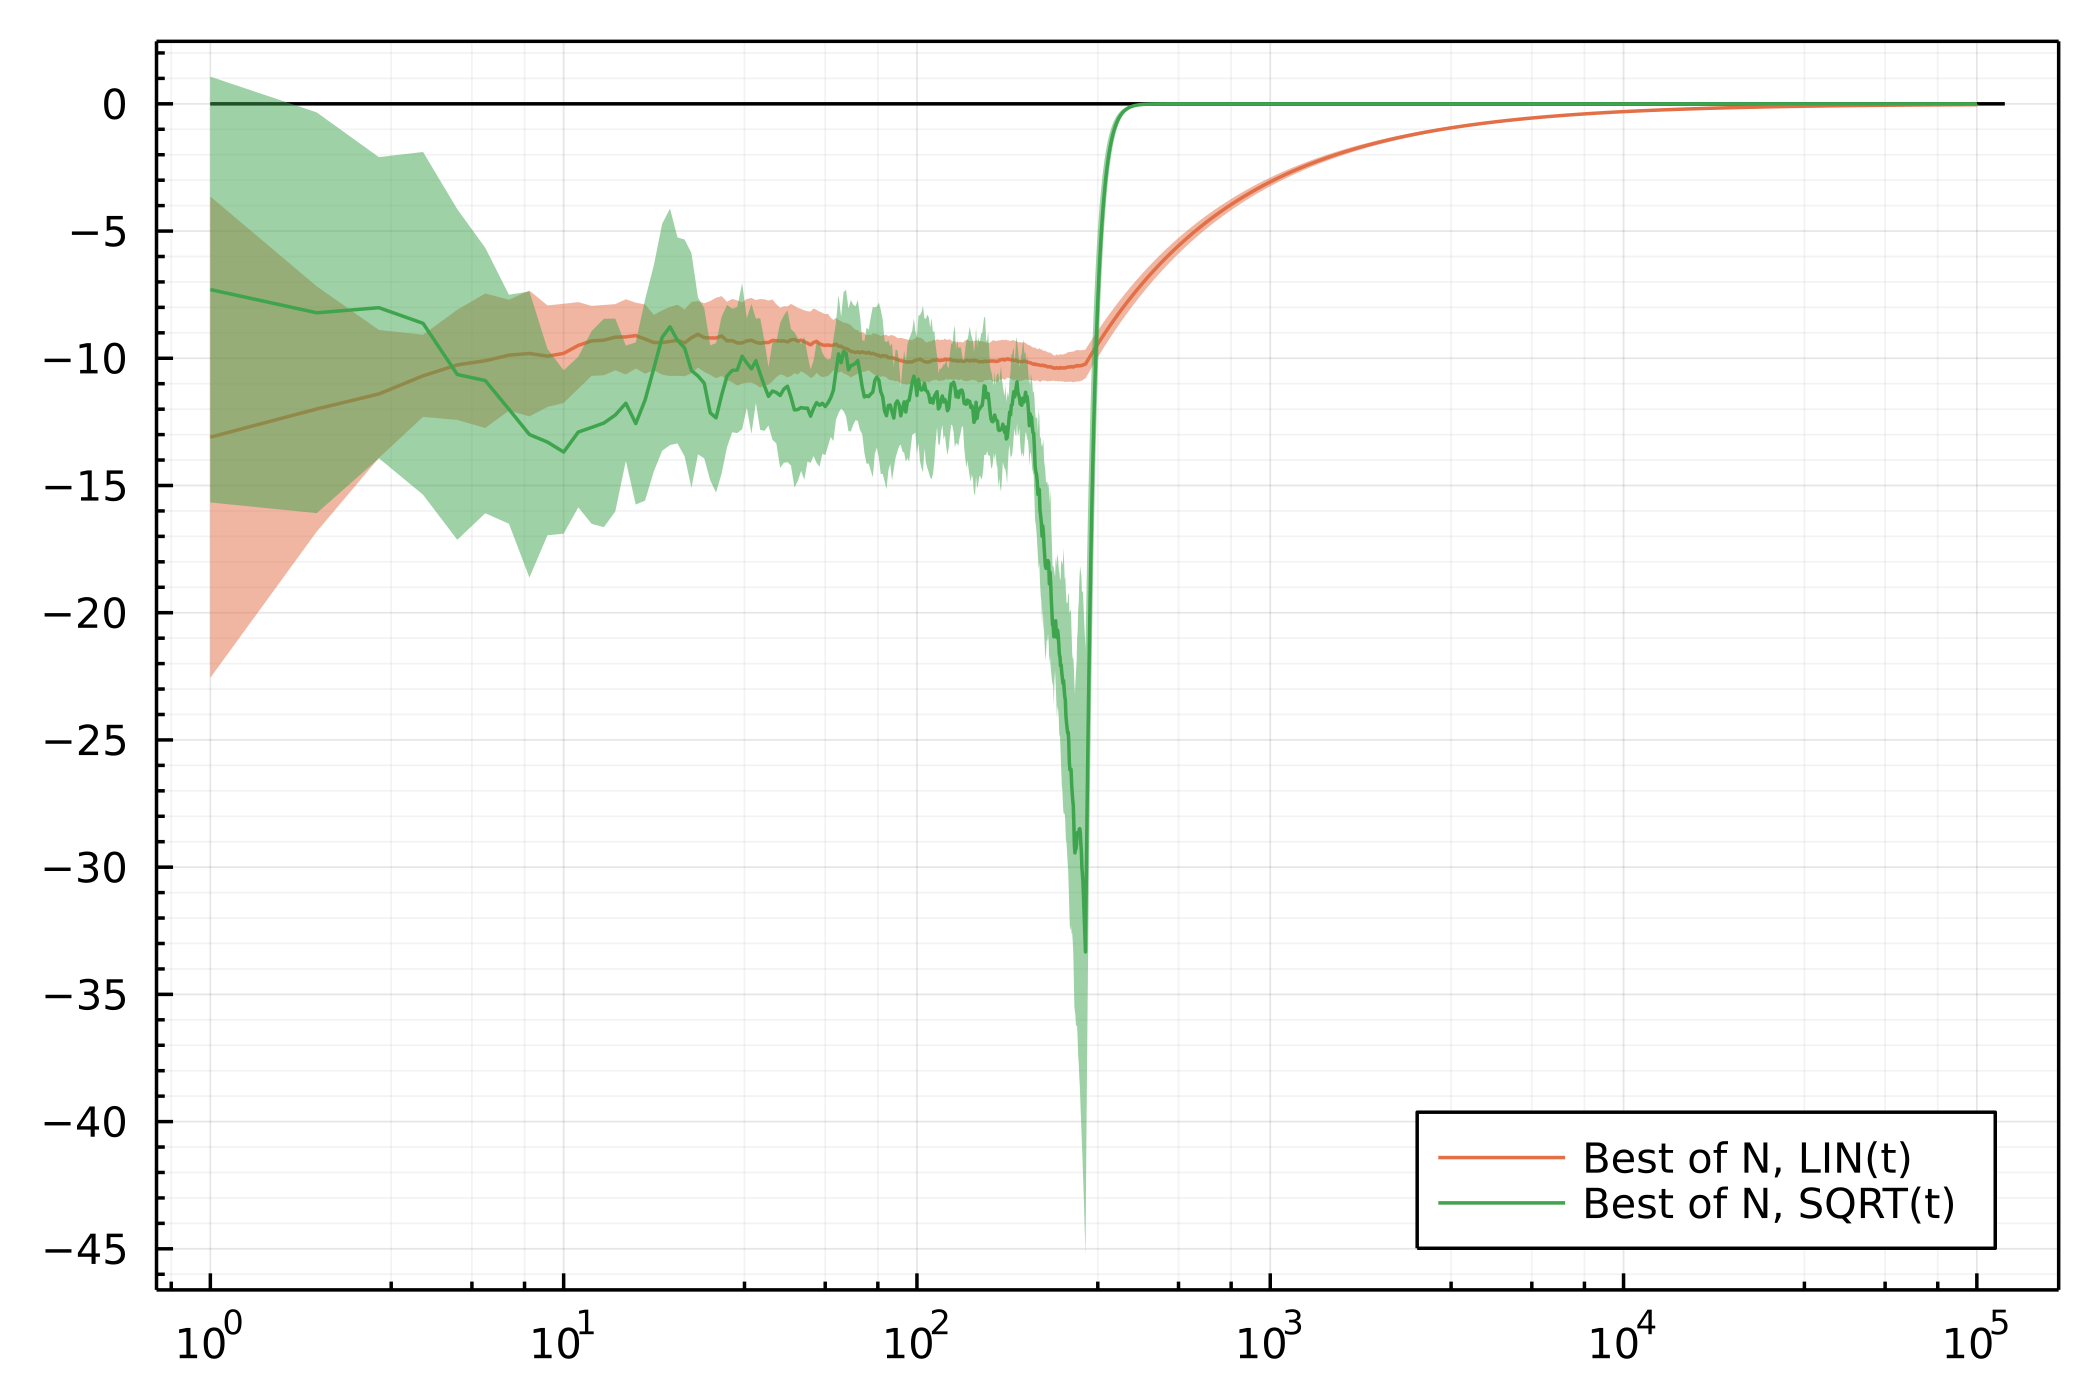
\includegraphics[width=1\textwidth]{sg/bestofn/tag_3_01_BestOfN_LinT_SqrtT_1_1.png}
        \caption{\tagname{3}{01} in state $s = \left(1, 1\right)$}
        \label{apx:sgexp:bestofn:fig:pure}
    \end{subfigure}
    \hfill
    \begin{subfigure}[t]{0.45\linewidth}
        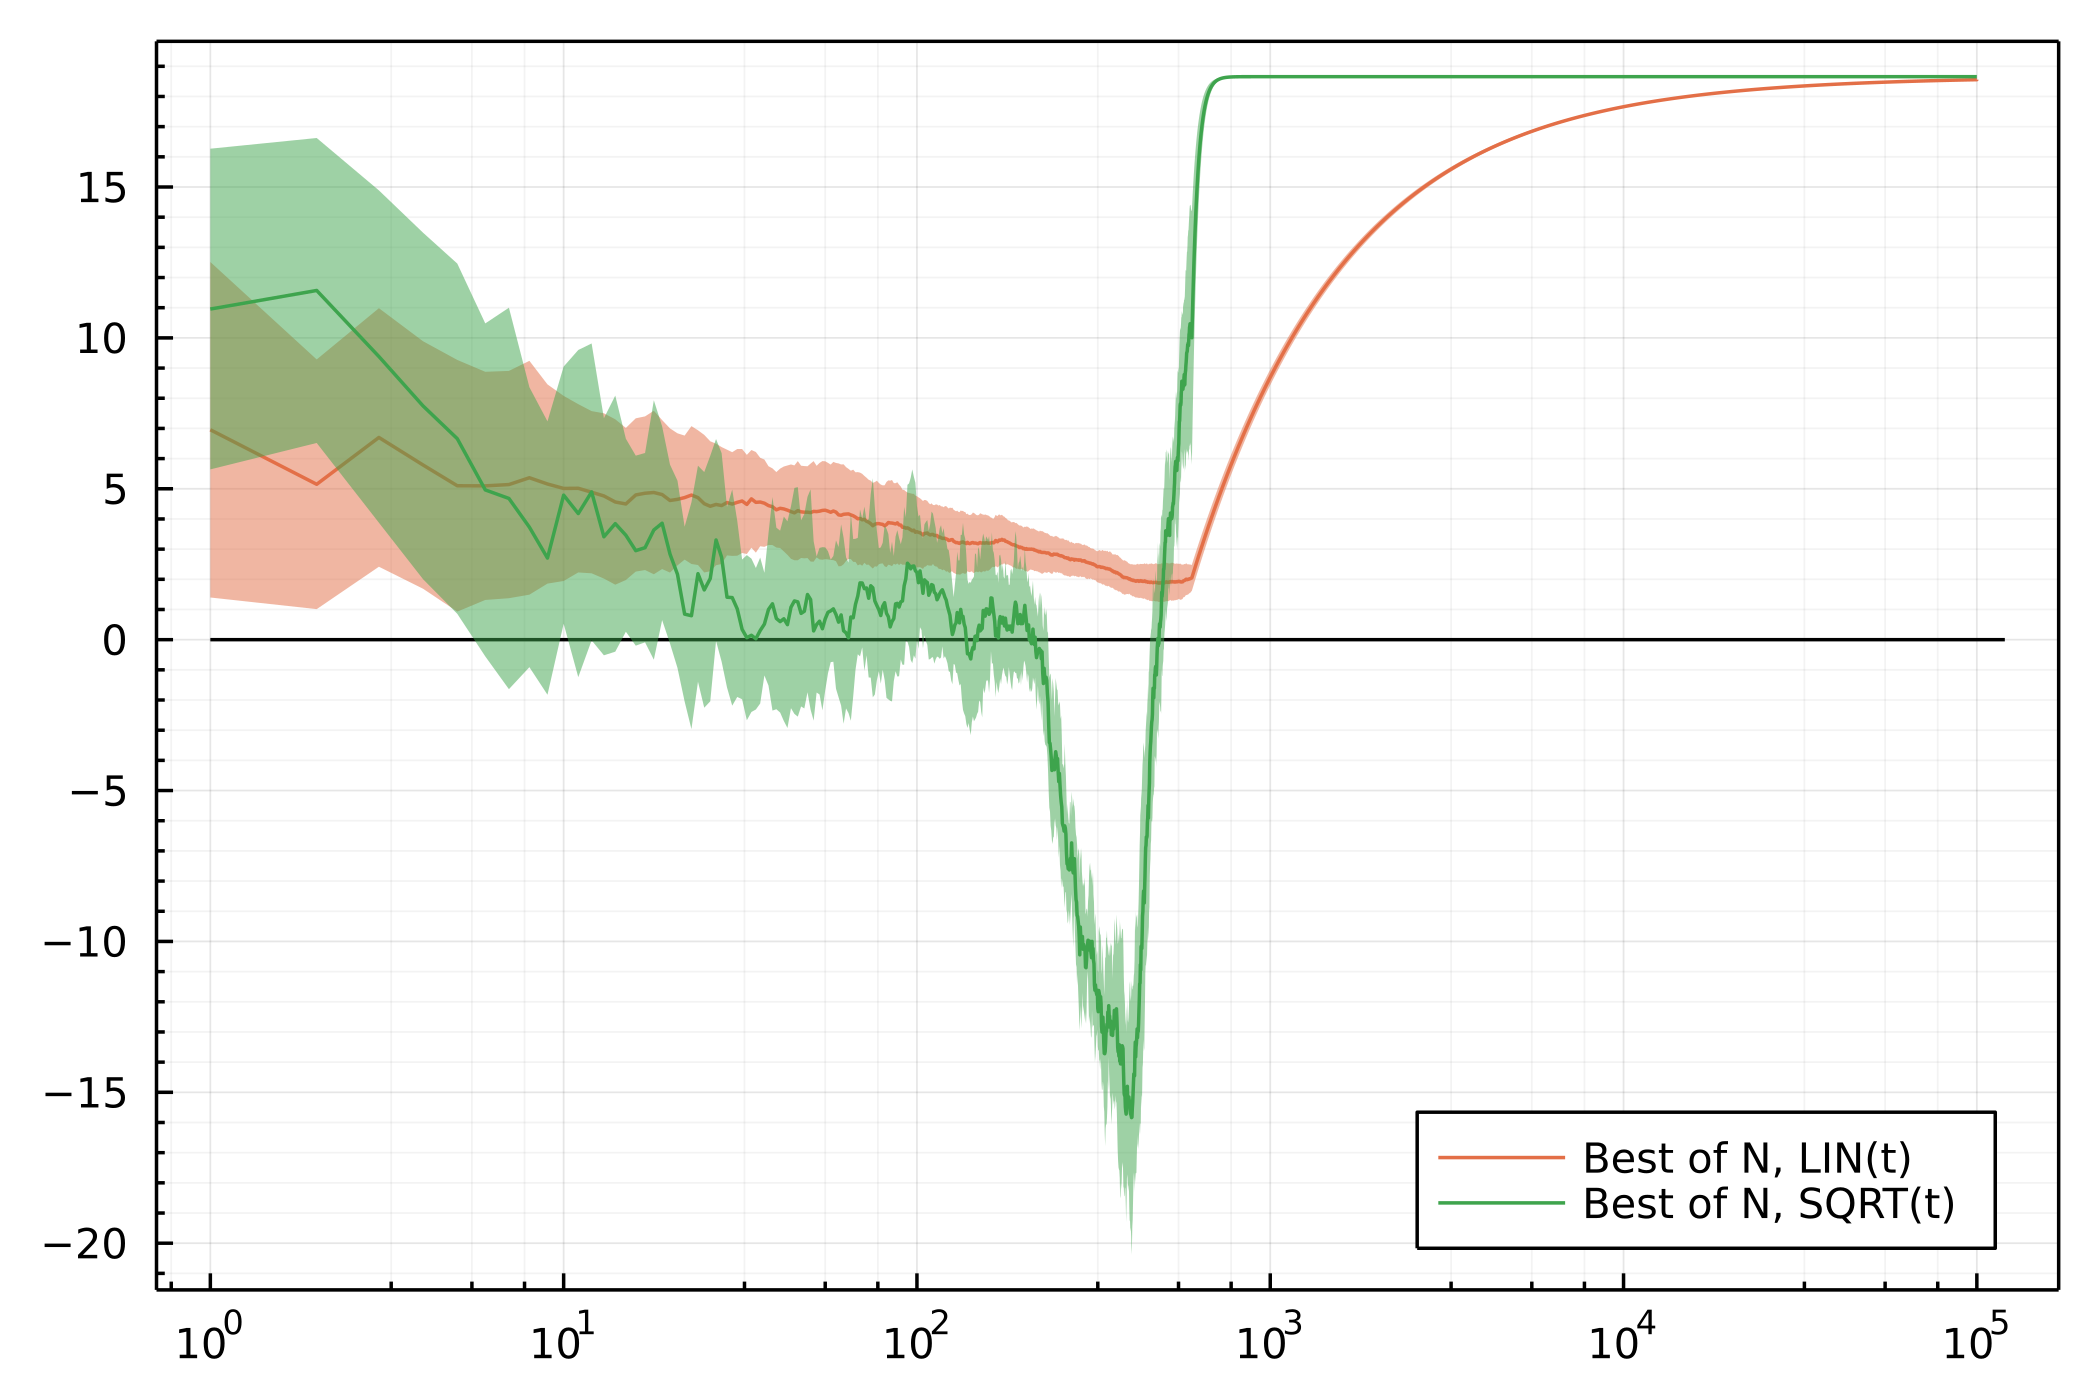
\includegraphics[width=1\textwidth]{sg/bestofn/tag_3_02_BestOfN_LinT_SqrtT_4_4.png}
        \caption{\tagname{3}{02} in state $s = \left(4, 4\right)$}
        \label{apx:sgexp:bestofn:fig:mixed}
    \end{subfigure}
    \caption[Performance of the Best of $N$ bandit on instances of \textbf{Tag}]{
        The two graphs depict performance of the Best of $N$ bandit, for $N = 100$, in starting states of two \textbf{Tag} instances, namely \tagname{3}{01} and \tagname{3}{02}.
        The left figure belongs to a state where the optimal strategy is pure, conversely the right figure to a starting state with mixed optimal strategy.
        The graphs represent the development of deviation of the returned value from the true optimal value in each iteration $t \in [0, 10^5]$.
        A comparison of the two step functions is displayed and in detail described in \ref{apx:sgexp:bestofn}.
    }
    \label{apx:sgexp:bestofn:fig}
\end{figure}
Graphs \reffig{apx:sgexp:bestofn:fig} depict, that after the first random search over all actions, until each was tried $N$ times, the bandit found the single best pure strategy and played it to the end, thus receiving the same reward forever.

The first state is from the instance \tagname{3}{01}, where both the tagger and the evader are located on position $1$ so a joint state $s = \left(1, 1\right)$.
The map of this game \reffig{exp:sg:games:tag:examples:31} suggests, that the optimal strategies of both players are pure.
The evader can only go down and thus the tagger can always hit him with the beam by shooting vertically.
The graph \reffig{apx:sgexp:bestofn:fig:pure} confirms that the Best of N bandit can and will find such a pure best actions for sufficiently large $N$ and converge to the optimal value.

On the contrary, the second state $\left(4, 4\right)$ from \tagname{3}{02} \reffig{exp:sg:games:tag:examples:32} has mixed optimal strategies.
Neither player can commit to play a single action, because the adversary would exploit this information and obtain better outcome than in the case of a randomized strategy.
For the evader, all directions are equally good and the tagger has to decide the direction of the beam as he is always able to hit the evader.
But clearly he has to randomize, because he cannot know the direction of the evader.
This can be verified by extracting the strategies from the value iteration algorithm, where the tagger chooses the beam direction with uniform probability.
The chart in \reffig{apx:sgexp:bestofn:fig} confirms the intuitive idea, that the Best of N bandit is not able to find the optimal value and converges to a different value.
The deviation improves over the course of the random search, but once the single pure action is selected, the value recedes from the optimum.

\subsection{Steps}
From the graphs in previous subsection, we can also compare the two types of steps, $\lint$ and $\sqrtt$.
The increased weights for the newer presumably more accurate values have no real benefit here.
Although, the $\sqrtt$ converges to the resulting value much faster during the initial random phase, both of these step methods eventually converge to the same value.
On the other hand, during the random search at the beginning, the $\sqrtt$ step deviates much farther.

\subsection{Observable variant}
As displayed in the example state plotted in \reffig{apx:sgexp:bestofn:fig:obs}, the observable variant behaves almost exactly the same as the standard bandit algorithm.
\begin{figure}[ht]
    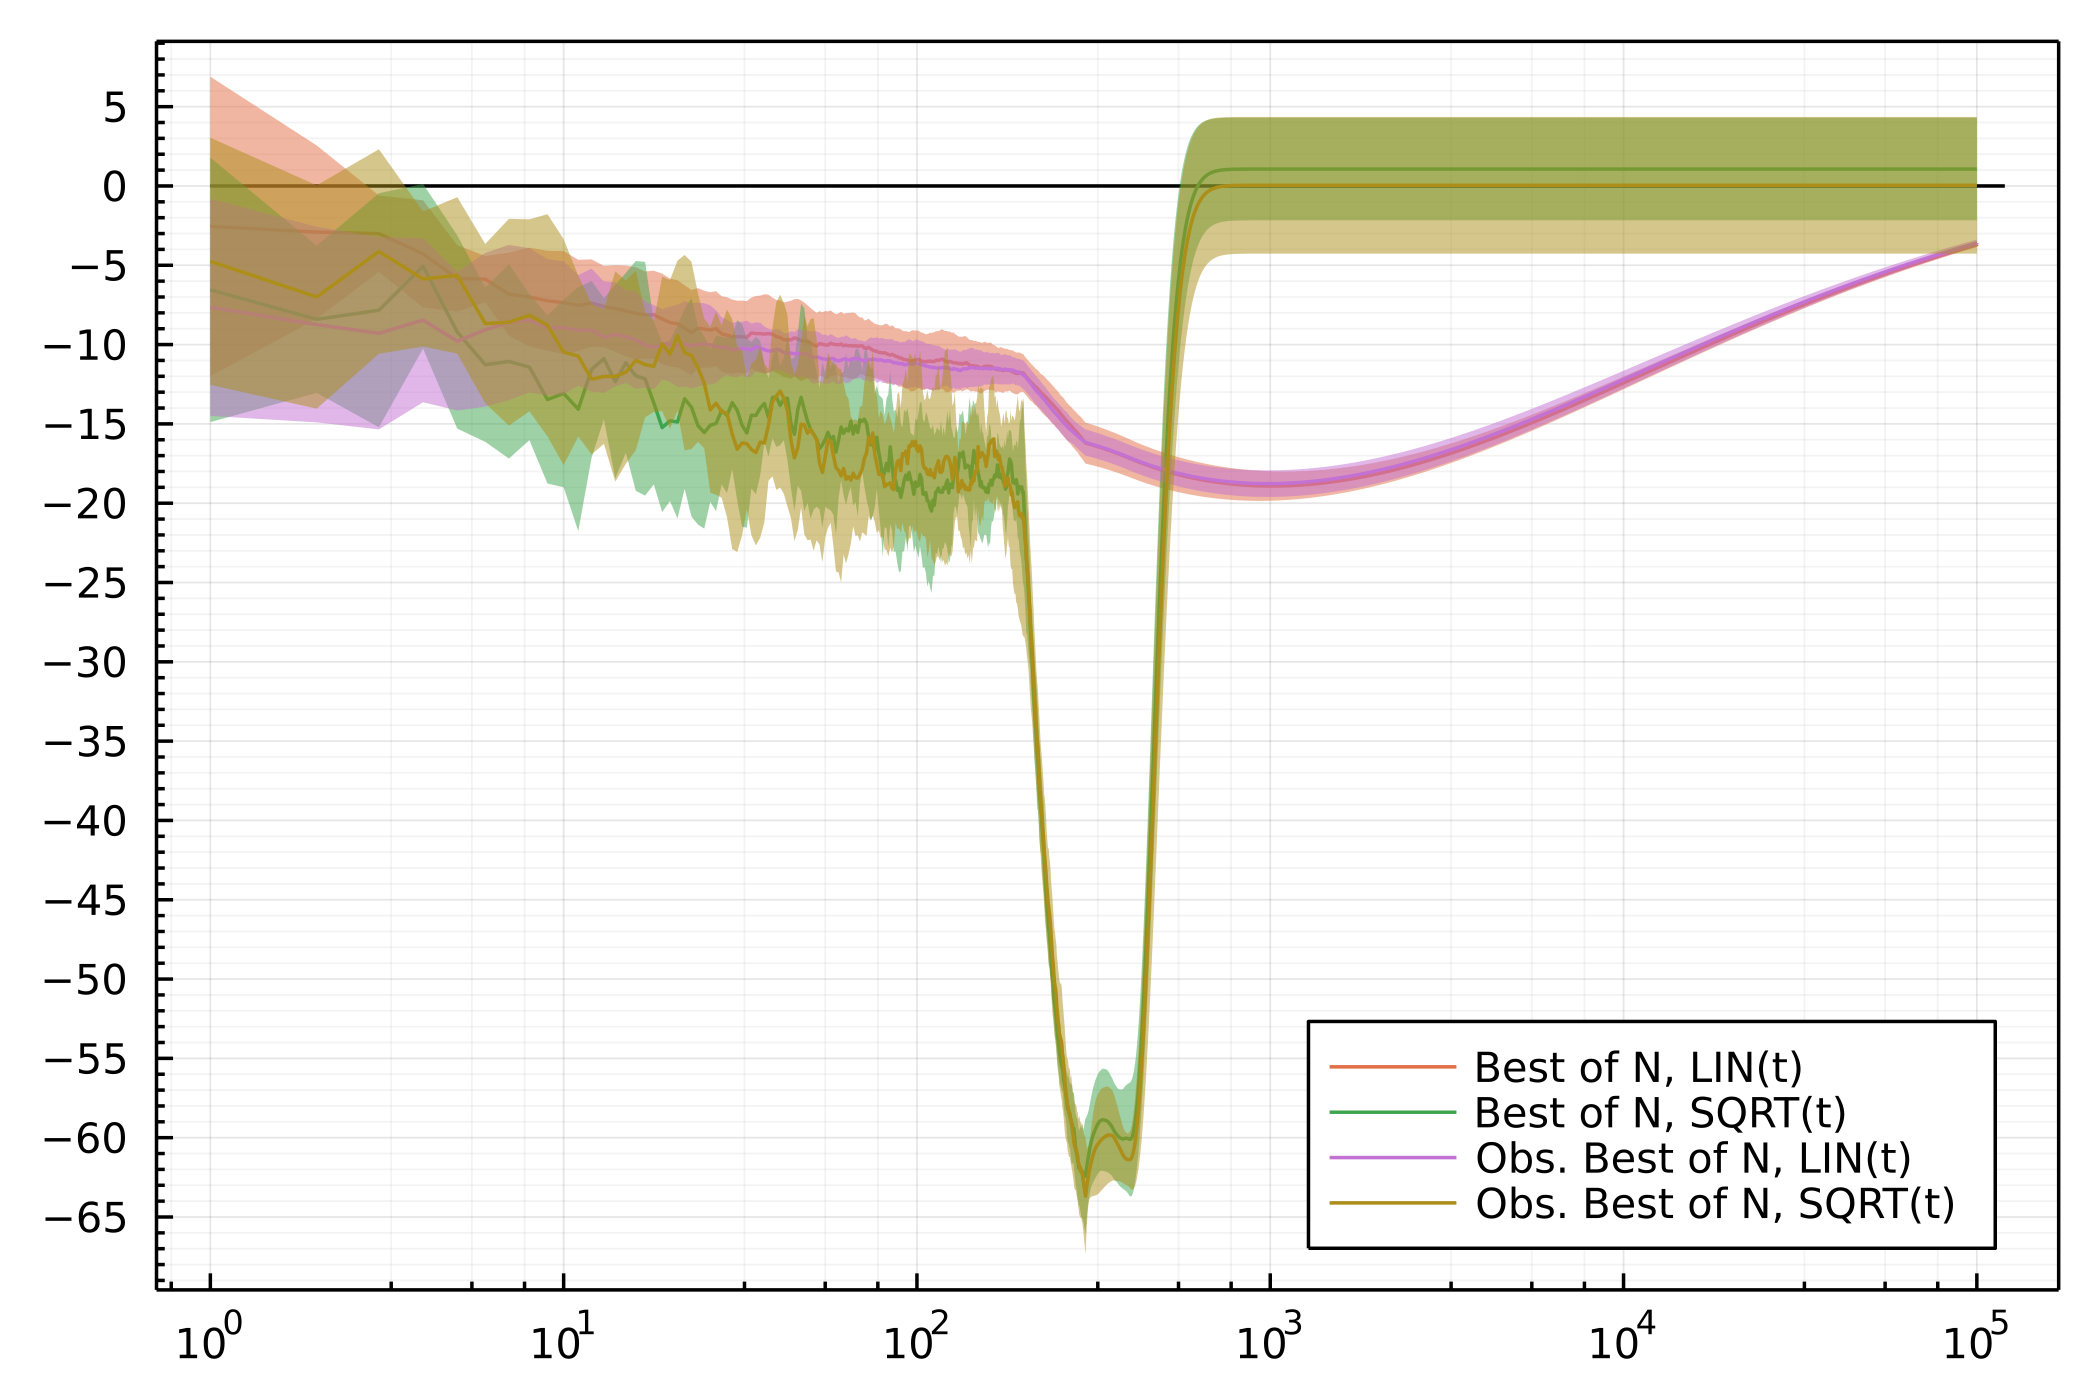
\includegraphics[width=0.8\textwidth]{sg/bestofn/tag_3_01_BestOfN_ObservableBestOfN_LinT_SqrtT_1_3.png}
    \caption[Comparison of standard and observable Best of $N$ bandit]{
        The figure shows comparison deviations from ground truth of the observable and non-observable variant of the Best of $N$ bandit on the instance \tagname{3}{01} in a joint initial state $s = \left(1, 3\right)$.
        It includes both types of step functions, $\lint$ and $\sqrtt$.
        The $x$ axis represents iterations of the bandit iteration algorithm.
    }
    \label{apx:sgexp:bestofn:fig:obs}
\end{figure}
Here, the average play of the adversary matters only once and that is in the selection of the best action after each was tried $N$ times.
But, at that moment the average play is a uniform strategy, so it does not have any effect on ruling out less promising options. 
Other choices are either completely random or conversely fixed to a single action.
Even though, from the graph it looks that the observable bandit converged exactly to the optimum, the intervals of standard deviation almost completely overlap and thus it cannot be confidently said that one reached the optimum while the other did not.

\section{$\epsilon$-greedy}\label{apx:sgexp:eps}
The second bandit algorithm for analysis is $\epsilon$-greedy.
Be reminded, that the search parameter was posed to $\epsilon = 0.1$.

\subsection{Convergence with average step LIN$(t)$}
In this part we consider only the averaging step LIN$(t)$, the other one will be discussed separately.

The $\epsilon$-greedy does not have a problem in getting close to the correct values in easy states with pure optimal strategies.
Although, it did not converge exactly to the value iteration results for states with many actions and randomized decisions (thus more difficult to learn the strategies precisely), based on the demonstrated trend of the deviation going towards zero, it would eventually converge given many more iterations.
The figure \reffig{apx:sgexp:eps:fig:hard} displays one easy and one hard state and the convergence in those respective states.
It displays states $s_1 = \left(4, 4\right)$ of the instance \tagname{3}{02} \reffig{exp:sg:games:tag:examples:32} and $s_2 = \left(4, 3\right)$ in the \chasename{5} instance \reffig{exp:sg:games:chase:examples:5}.
\begin{figure}[ht]
    \begin{subfigure}[t]{0.45\linewidth}
        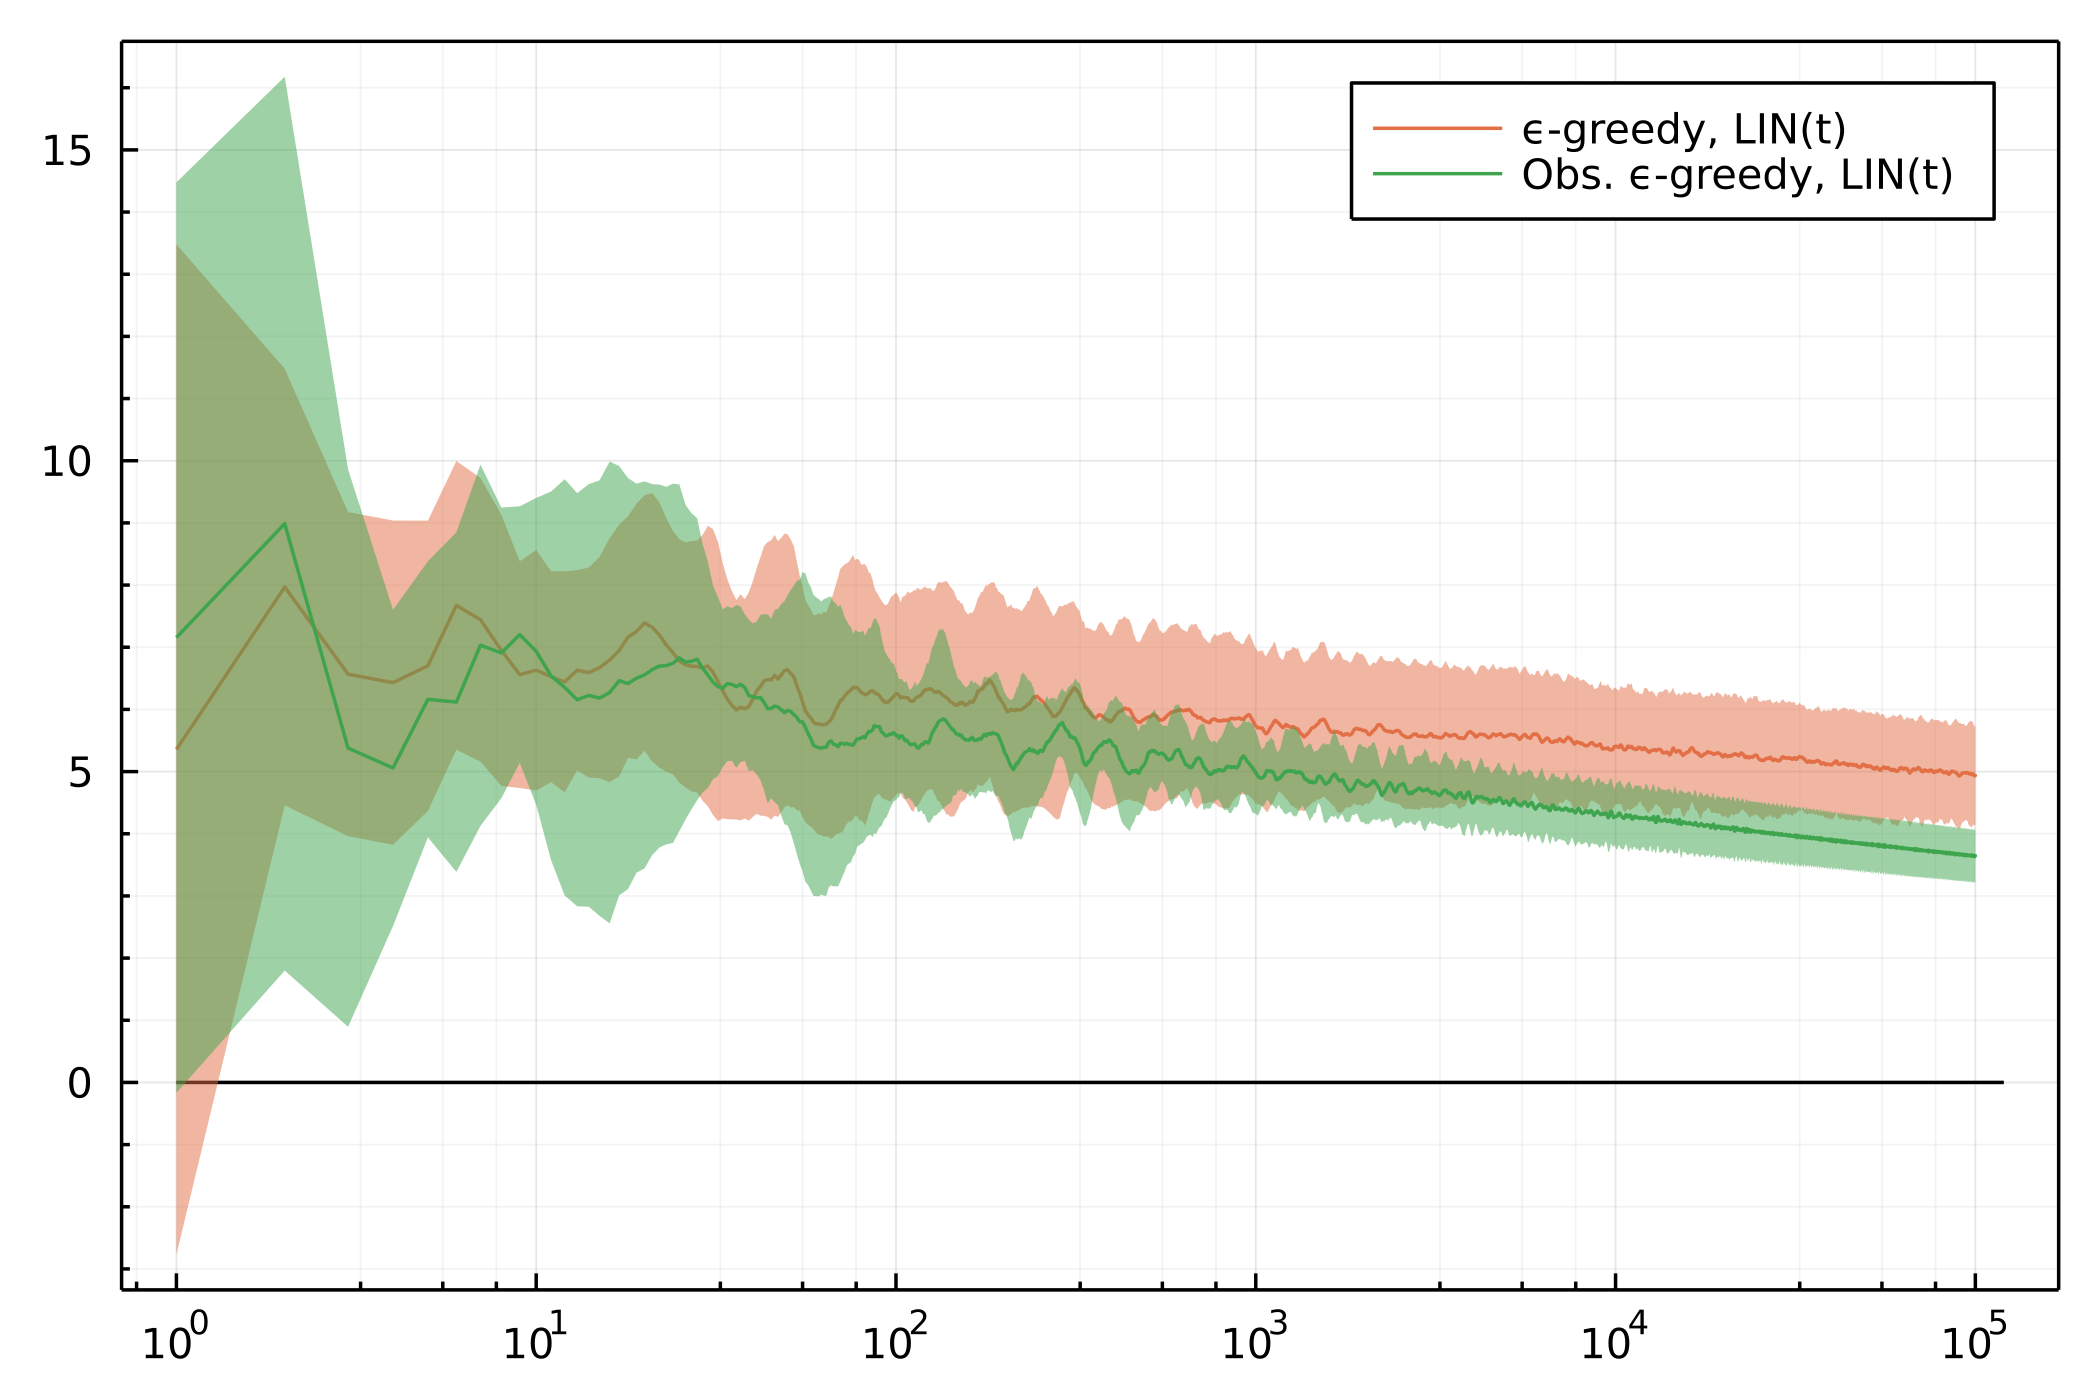
\includegraphics[width=1\textwidth]{sg/egreedy/tag_3_02_EpsilonGreedy_ObservableEpsilonGreedy_LinT_4_4.png}
        \caption{\tagname{3}{02} in state $s = \left(4, 4\right)$}
        \label{apx:sgexp:eps:fig:tag:44}
    \end{subfigure}
    \hfill
    \begin{subfigure}[t]{0.45\linewidth}
        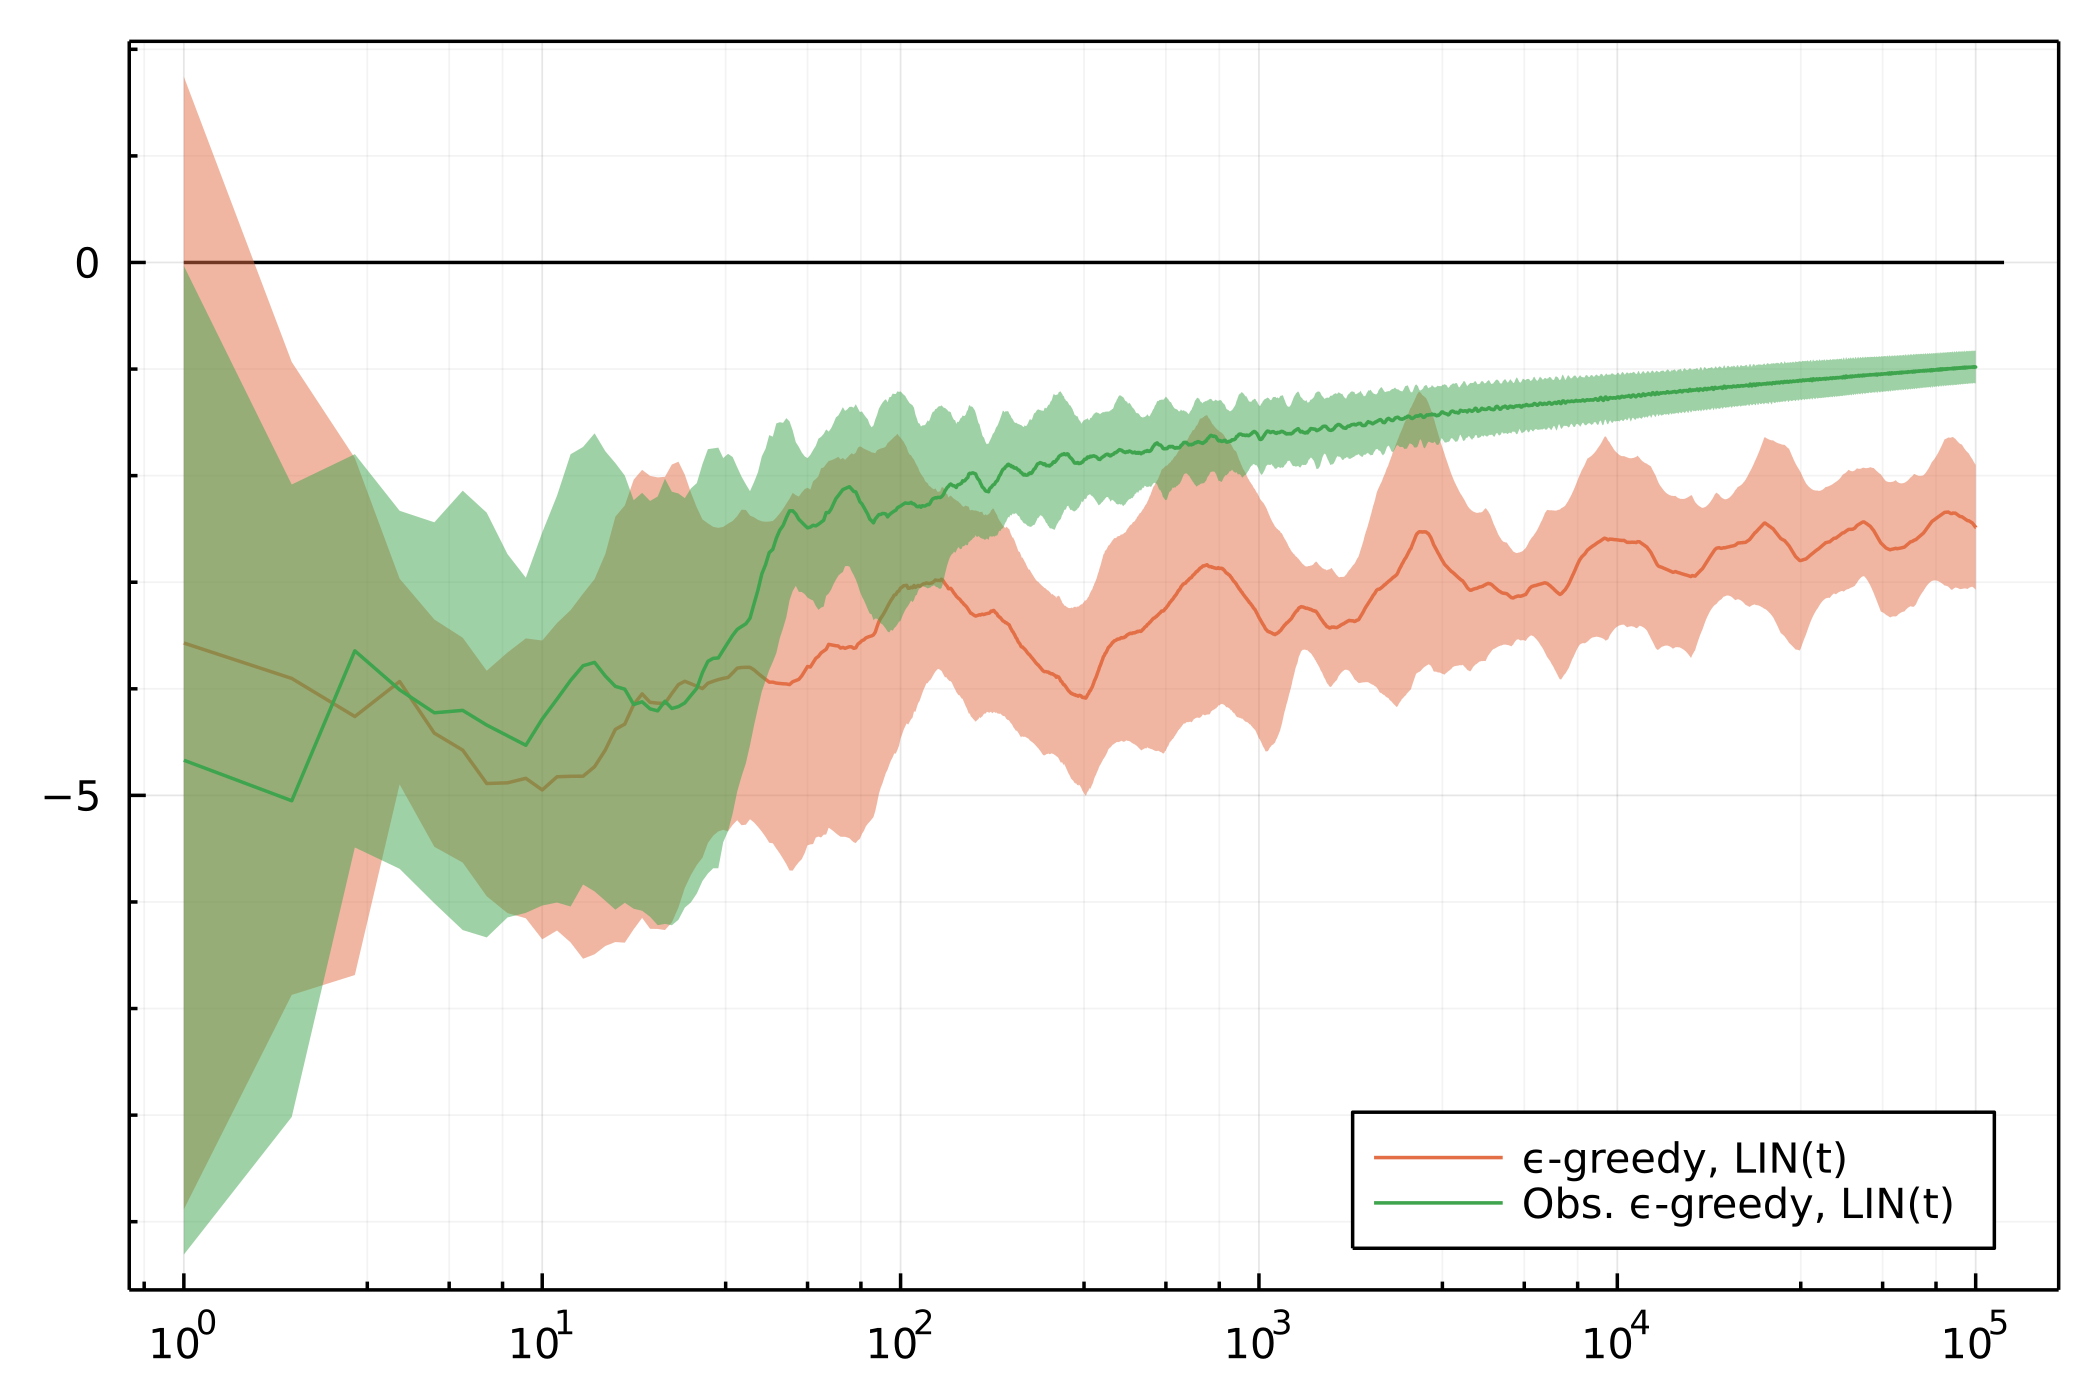
\includegraphics[width=1\textwidth]{sg/egreedy/graphs_5_01_EpsilonGreedy_ObservableEpsilonGreedy_LinT_4_3.png}
        \caption{\chasename{5} in state $s = \left(4, 3\right)$}
        \label{apx:sgexp:eps:fig:chase:43}
    \end{subfigure}
    \caption[$\epsilon$-greedy with $\lint$ learning mixed strategies]{
        These graphs display convergence of the $\epsilon$-greedy bandit algorithm to the values of states with mixed optimal strategies, when the $\lint$ step function is used to accumulate rewards.
        The $y$ axis represents deviation from the value iteration optimal value shown as a black graph of a constant function in each iteration on $x$ axis.
    }
    \label{apx:sgexp:eps:fig:hard}
\end{figure}
Moreover, from both of these figures, the observable variant outperforms the standard one and gets closer and faster to the optimum.
In contrast to the Best of N bandit \refsec{apx:sgexp:bestofn}, $\epsilon$-greedy selects best action 9 times out of 10 trials on average and thus the average play of the opponent influences the decisions in the observable variant.

\subsection{Accumulation step $\sqrtt$}
Generally, the $\epsilon$-greedy bandit struggles with the intensive exploration at the end, causing bigger fluctuations in the accumulated value.
This gets highlighted by the use of the step function $\sqrtt$.
The algorithm definitely gets closer to the optimal value than the $\lint$ but then, due to the quite frequent random decisions, the solution rather oscillates around the optimum.
However, in easy states, this averaging step is effective, especially with the employed average play.

The figures \reffig{apx:sgexp:eps:fig:sqrt} depict these two cases on the observable bandit.
\begin{figure}[ht]
    \begin{subfigure}[t]{0.45\linewidth}
        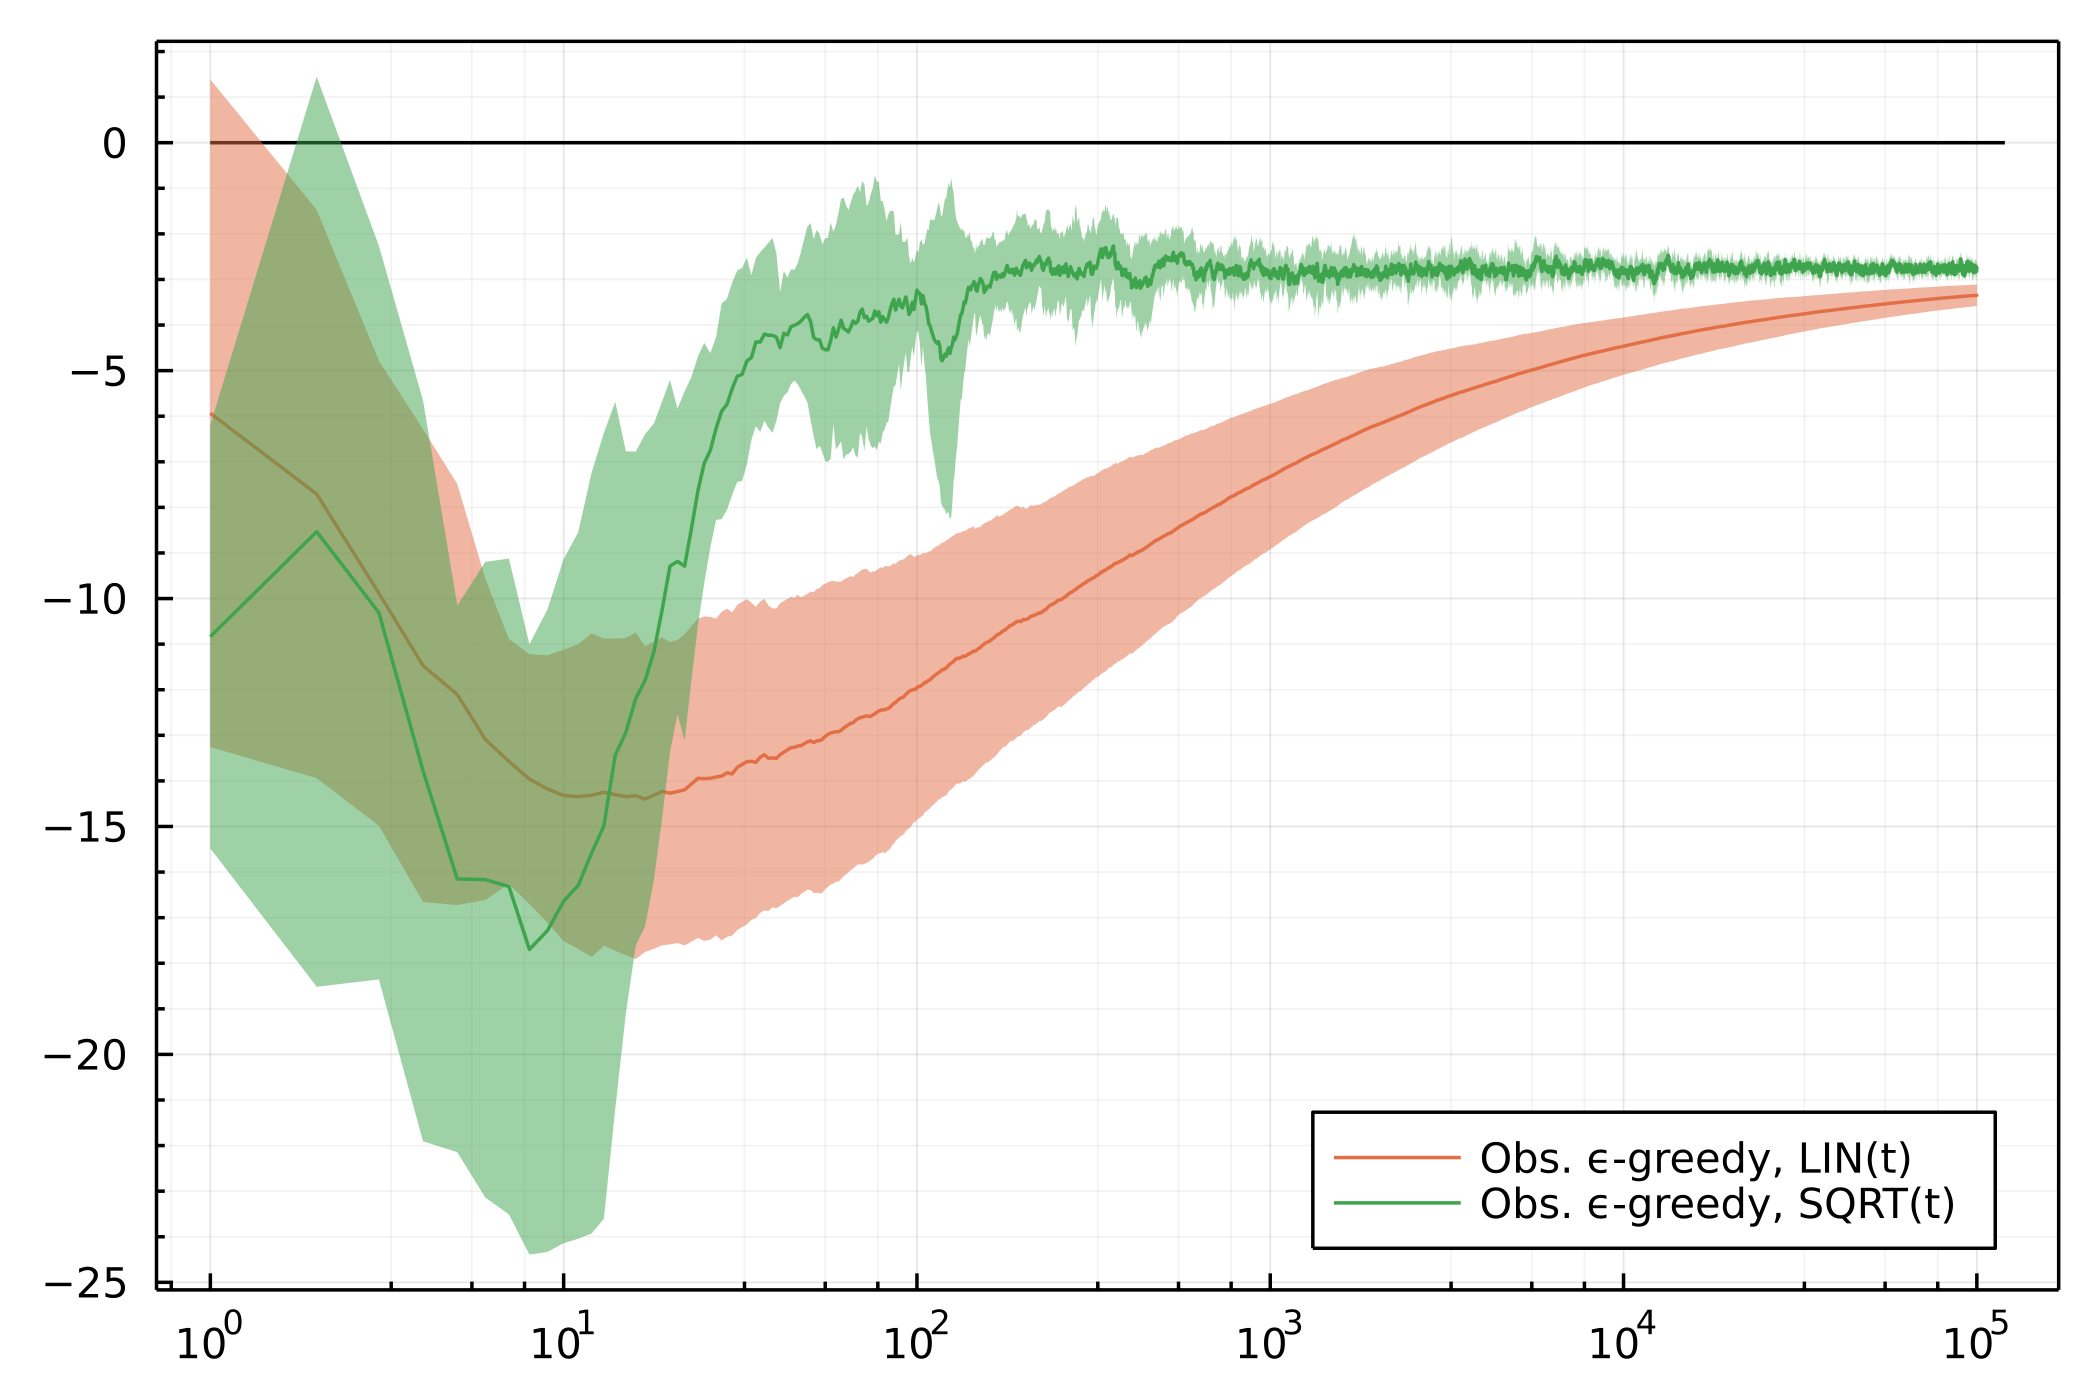
\includegraphics[width=1\textwidth]{sg/egreedy/tag_3_01_ObservableEpsilonGreedy_LinT_SqrtT_1_4.png}
        \caption{$\sqrtt$ outperforms $\lint$ on \tagname{3}{01} in $s = \left(1, 4\right)$}
        \label{apx:sgexp:eps:fig:sqrt:outperforms}
    \end{subfigure}
    \hfill
    \begin{subfigure}[t]{0.45\linewidth}
        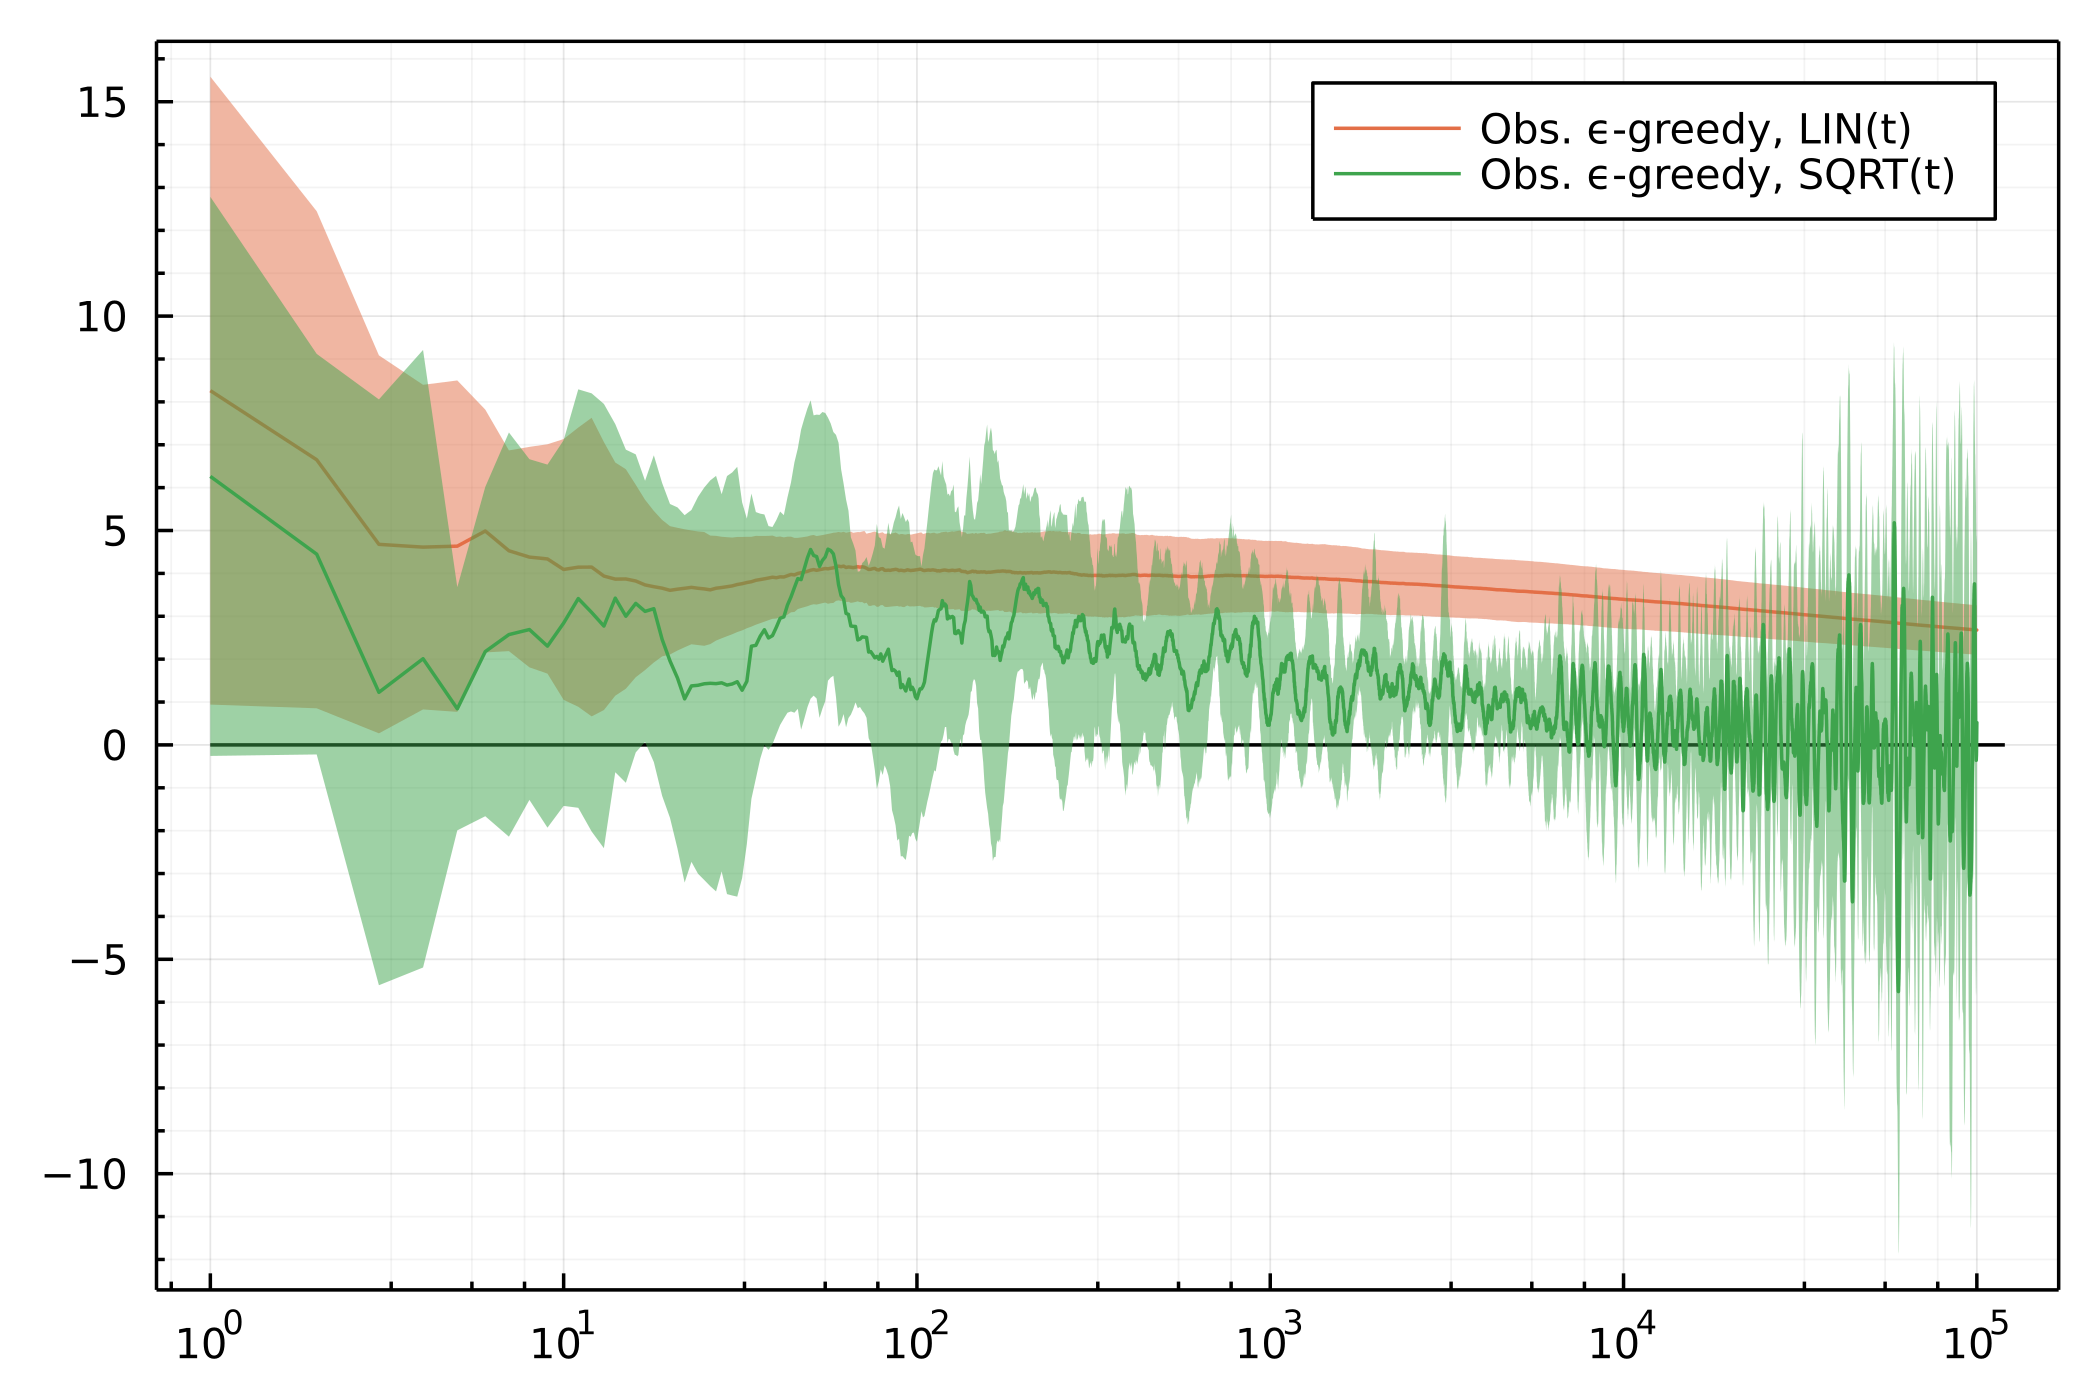
\includegraphics[width=1\textwidth]{sg/egreedy/tag_3_02_ObservableEpsilonGreedy_LinT_SqrtT_1_4.png}
        \caption{$\sqrtt$ oscillates in \tagname{3}{02} in $s = \left(1, 4\right)$}
        \label{apx:sgexp:eps:fig:sqrt:oscilates}
    \end{subfigure}
    \caption[Comparison of $\lint$ and $\sqrtt$ in combination with $\epsilon$-greedy bandit]{
        This chart compares the two step functions $\lint$ and $\sqrtt$ and how they influence performance of the $\epsilon$-greedy bandit in states with mixed optimal strategies.
        The performance is measured as a dependence of difference between the optimal value and the value from bandit iteration on iterations $t$.
    }
    \label{apx:sgexp:eps:fig:sqrt}
\end{figure}

This makes the accumulation step $\sqrtt$ not very convenient for $\epsilon$-greedy, because the one random explorative action selection shifts the value more than is desirable.
This flaw could be improved by employing some adaptive way of setting $\epsilon$ for each iteration and cool down exploration in later rounds.

In the easiest states, the both step functions produce equivalent results.
For example, in states where only a single action is available for one of the players.

\section{Successive elimination}\label{apx:sgexp:succ}
The Successive elimination multi-armed bandit is the first examined algorithm, which adapts its behaviour based on the received rewards.
It should perform better in learning randomized strategies, but due to the deactivation of actions when the confidence intervals do not overlap, it can still degrade to pure strategy even though it was not optimal.
This also depends on the setting of the exploration parameter $\alpha$.

In the figures \reffig{apx:sgexp:succ:fig}, the extreme occurrences of the phenomenon described before are showcased.
\begin{figure}[ht]
    \begin{subfigure}[t]{0.45\linewidth}
        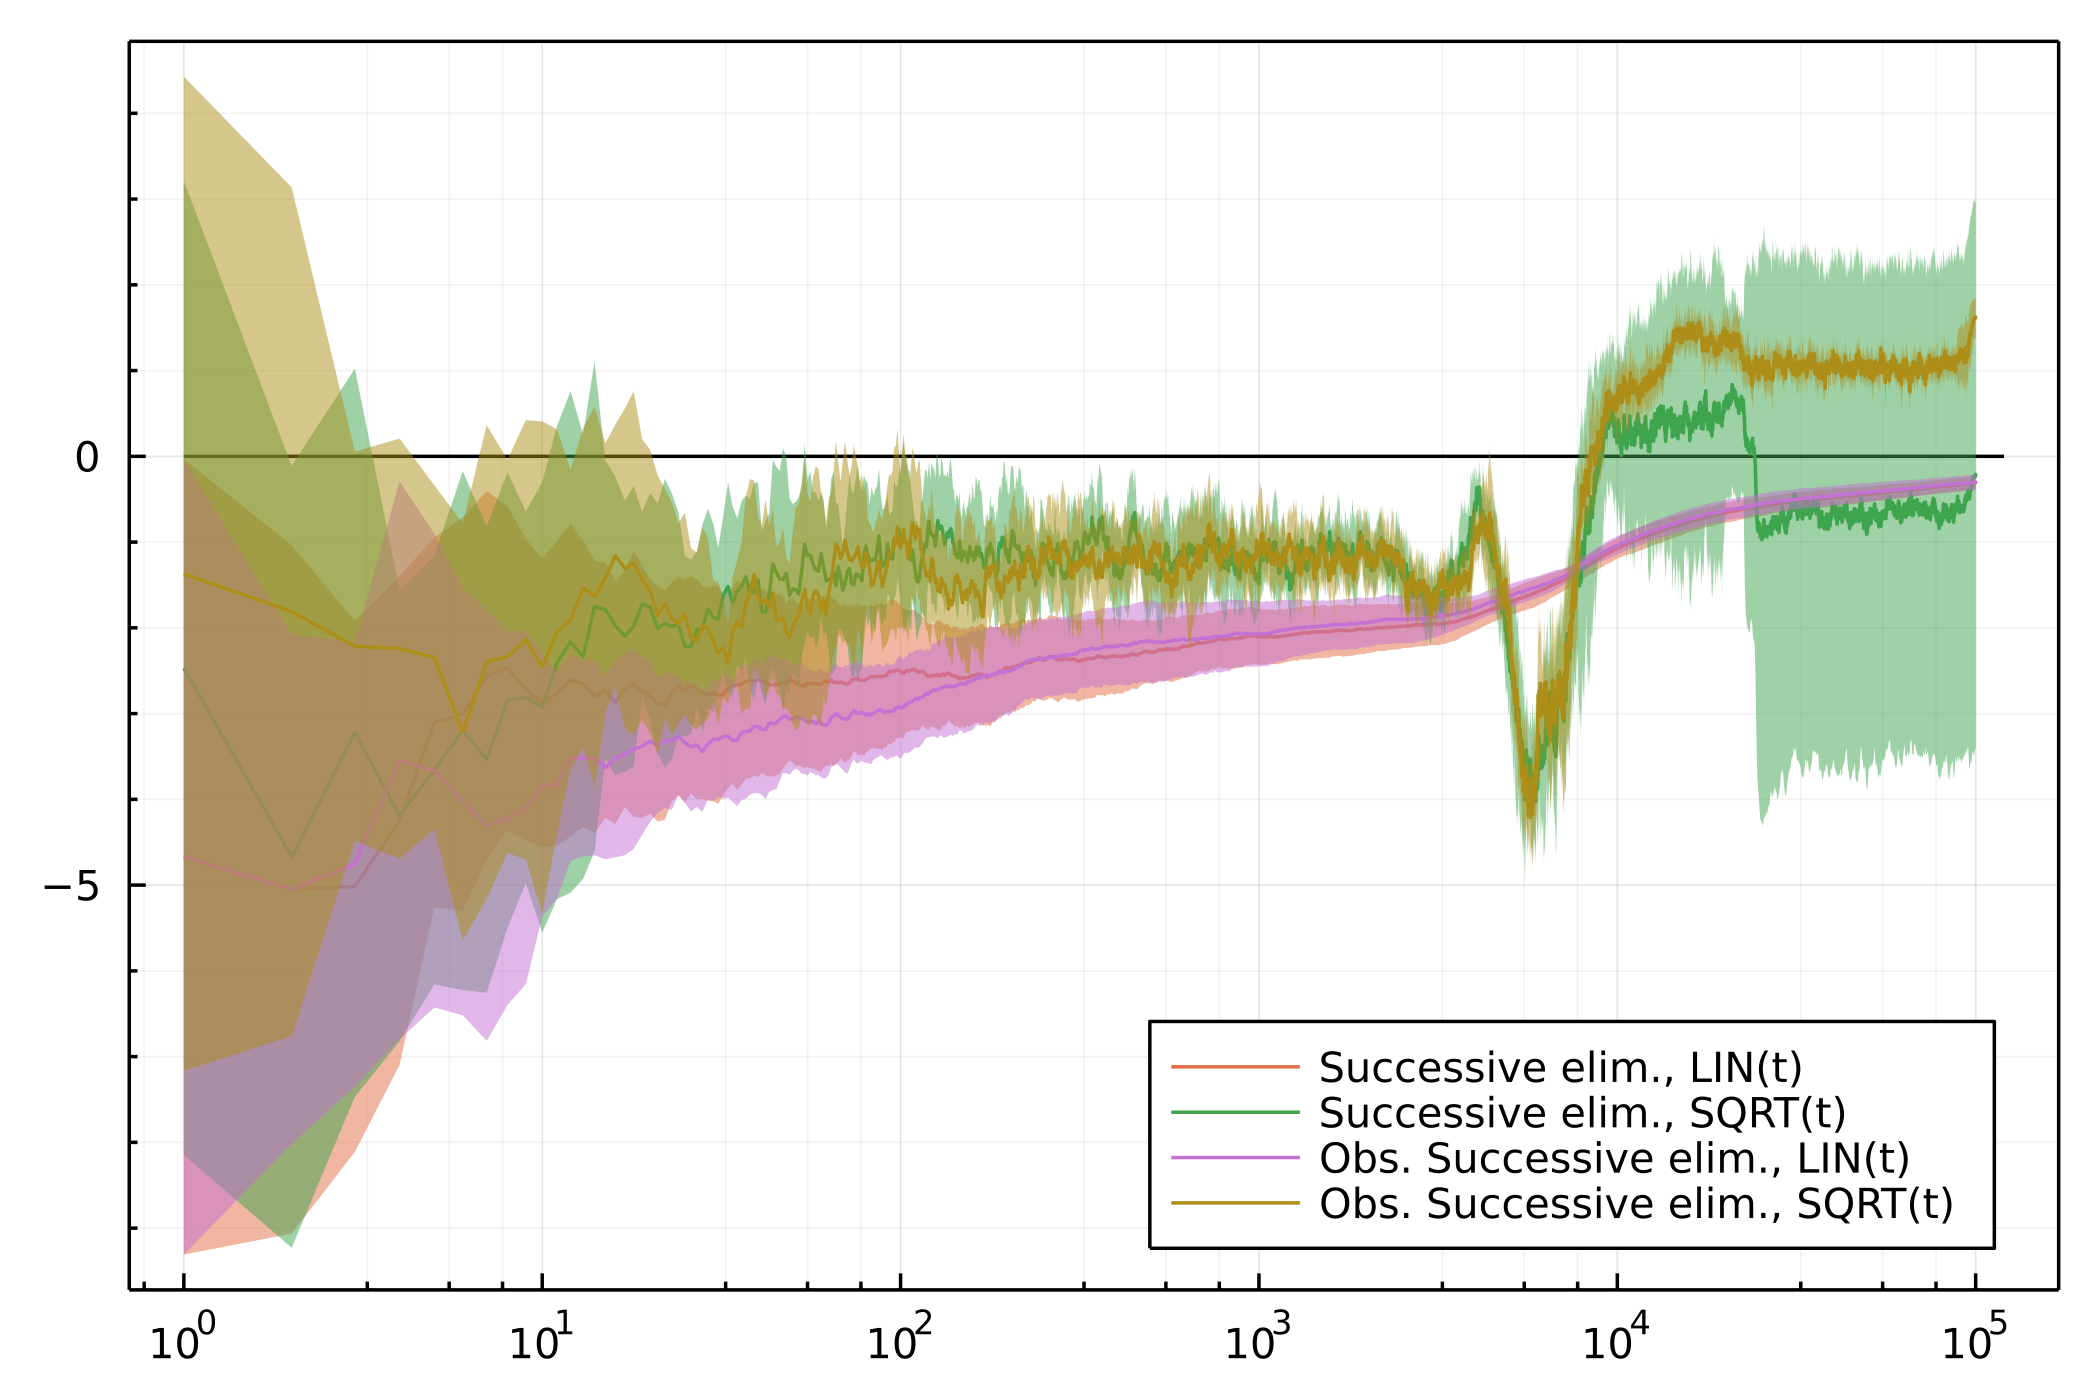
\includegraphics[width=1\textwidth]{sg/succ/graphs_5_01_SuccessiveElimination_ObservableSuccessiveElimination_LinT_SqrtT_4_3.png}
        \caption{Behaviour in joint state $s = \left(4, 3\right)$}
        \label{apx:sgexp:succ:fig:graph5:43}
    \end{subfigure}
    \hfill
    \begin{subfigure}[t]{0.45\linewidth}
        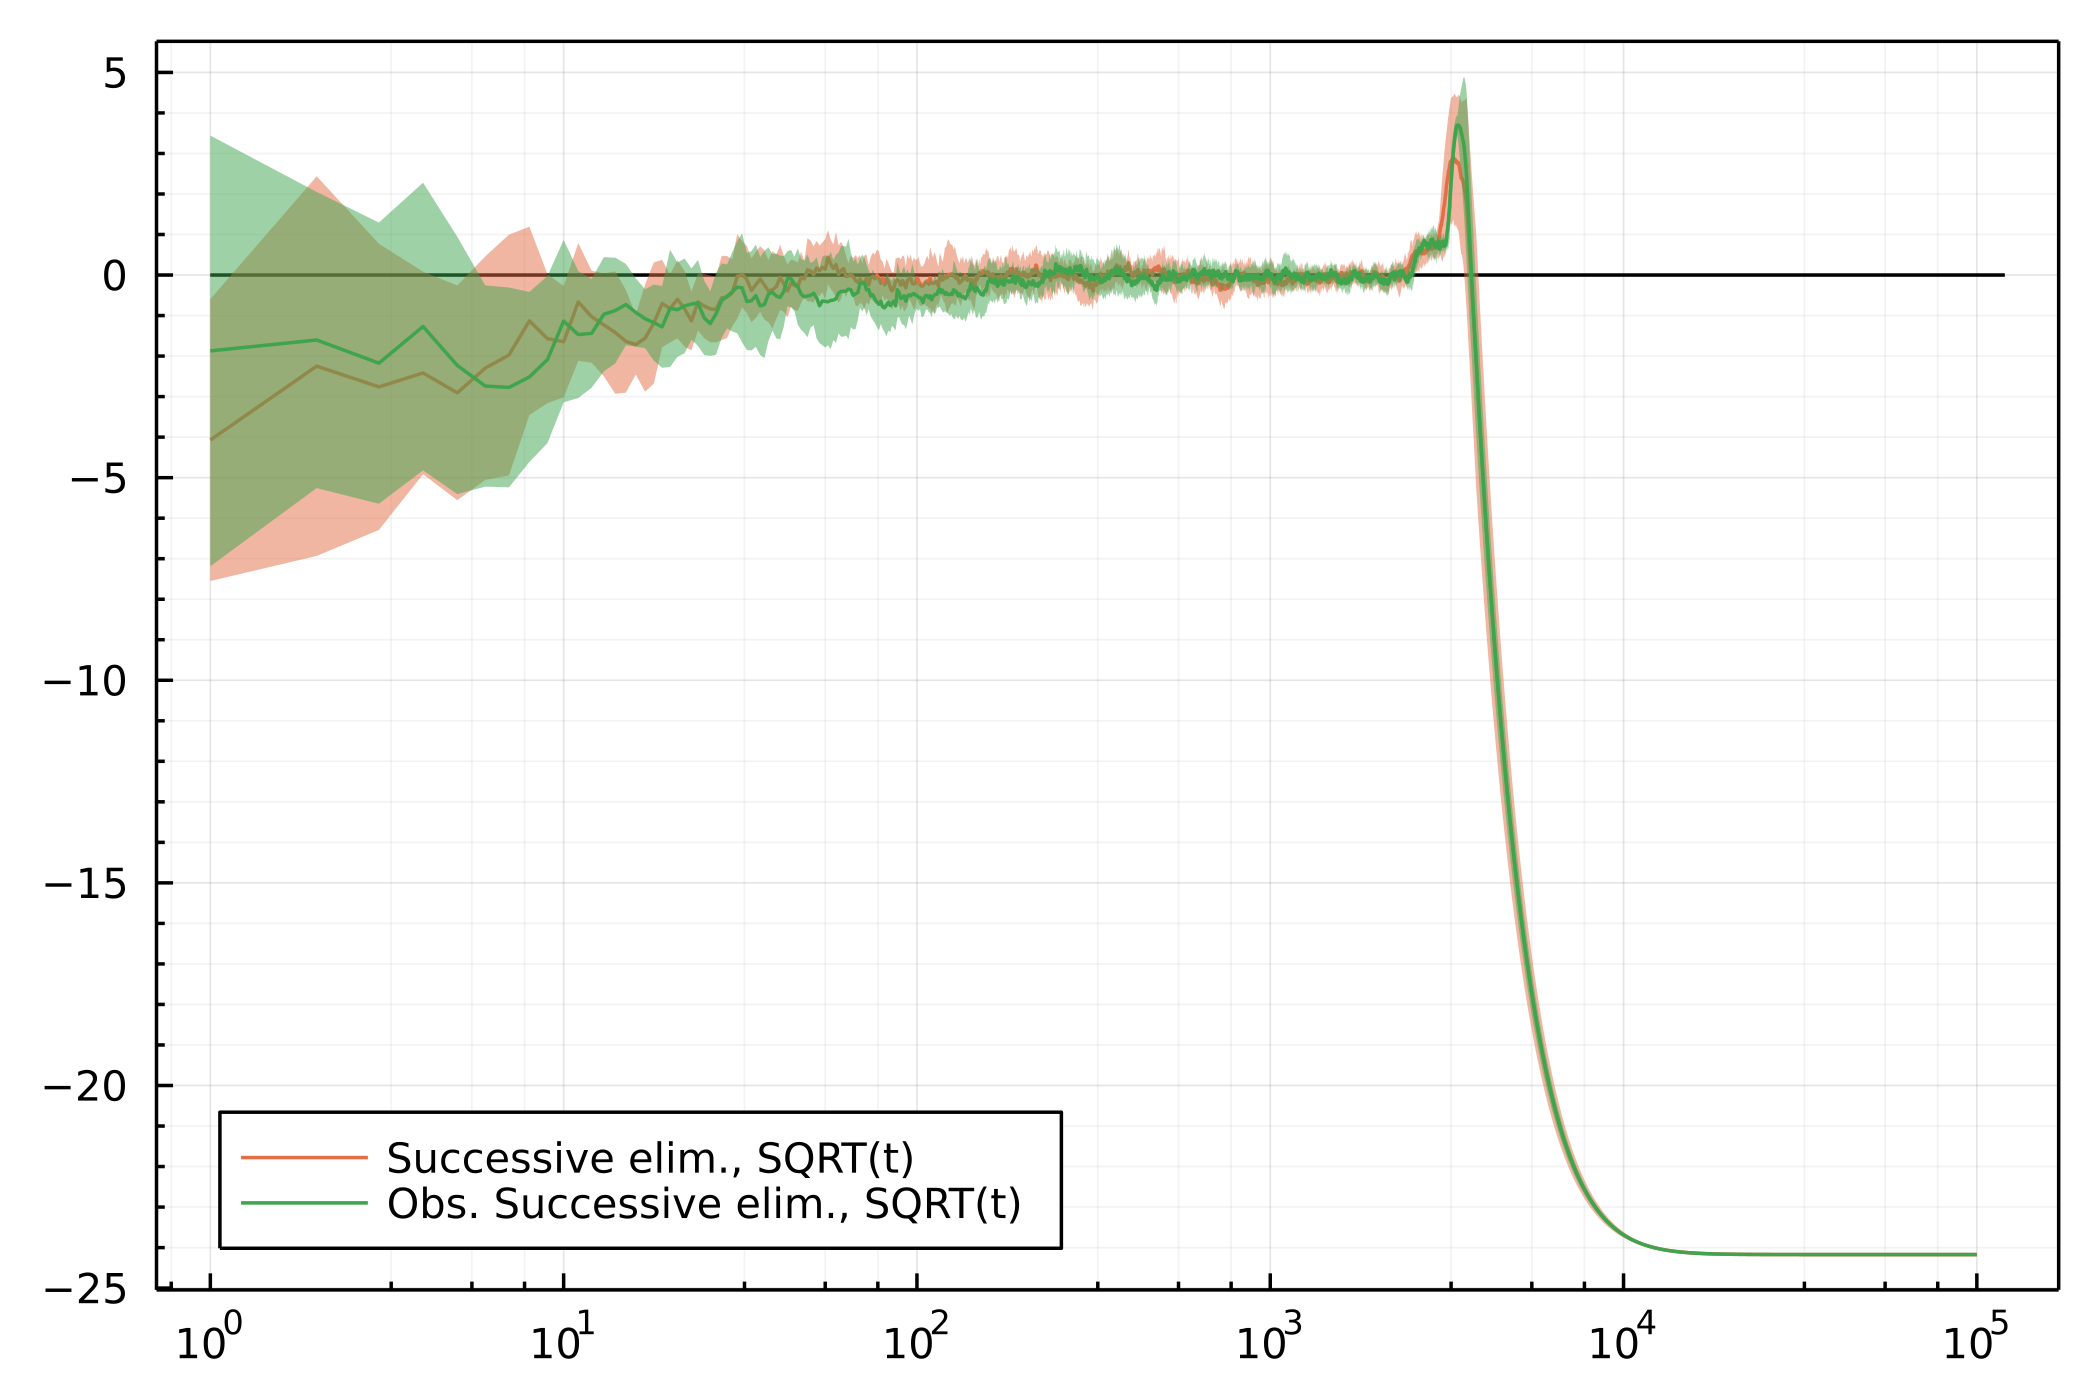
\includegraphics[width=1\textwidth]{sg/succ/graphs_5_01_SuccessiveElimination_ObservableSuccessiveElimination_SqrtT_2_1.png}
        \caption{Behaviour in joint state $s = \left(2, 1\right)$}
        \label{apx:sgexp:succ:fig:graph5:21}
    \end{subfigure}
    \caption[Comparison of observable and standard Successive elimination bandit]{
        The figures depict graphs of convergence of returned values of the Successive elimination multi-armed bandit when used with the bandit iteration on \chasename{5}.
        The learned values correspond to values read on the $y$ axis and the iterations of the framework on the $x$ axis.
    }
    \label{apx:sgexp:succ:fig}
\end{figure}
On the left figure \reffig{apx:sgexp:succ:fig:graph5:43}, we see an example, when the function $\lint$ slowly converges to the optimal value.
The $\sqrtt$, however, gets close very quickly but then some arm which was important in the mixed strategy gets deactivated and the value shifts somewhere else.
The rapid changes in the graph of the obtained values exactly correspond to deactivation of some arm by the bandit.
And while the $\lint$ function does not sway very much, the $\sqrtt$ step causes high fluctuations.

In the right figure \reffig{apx:sgexp:succ:fig:graph5:21}, the algorithm converged almost exactly to the optimal value, but after the important action is removed from the decisions, the value drifts afar.

An example of a situation when the deactivation rule benefits the learning.
\begin{figure}[ht]
    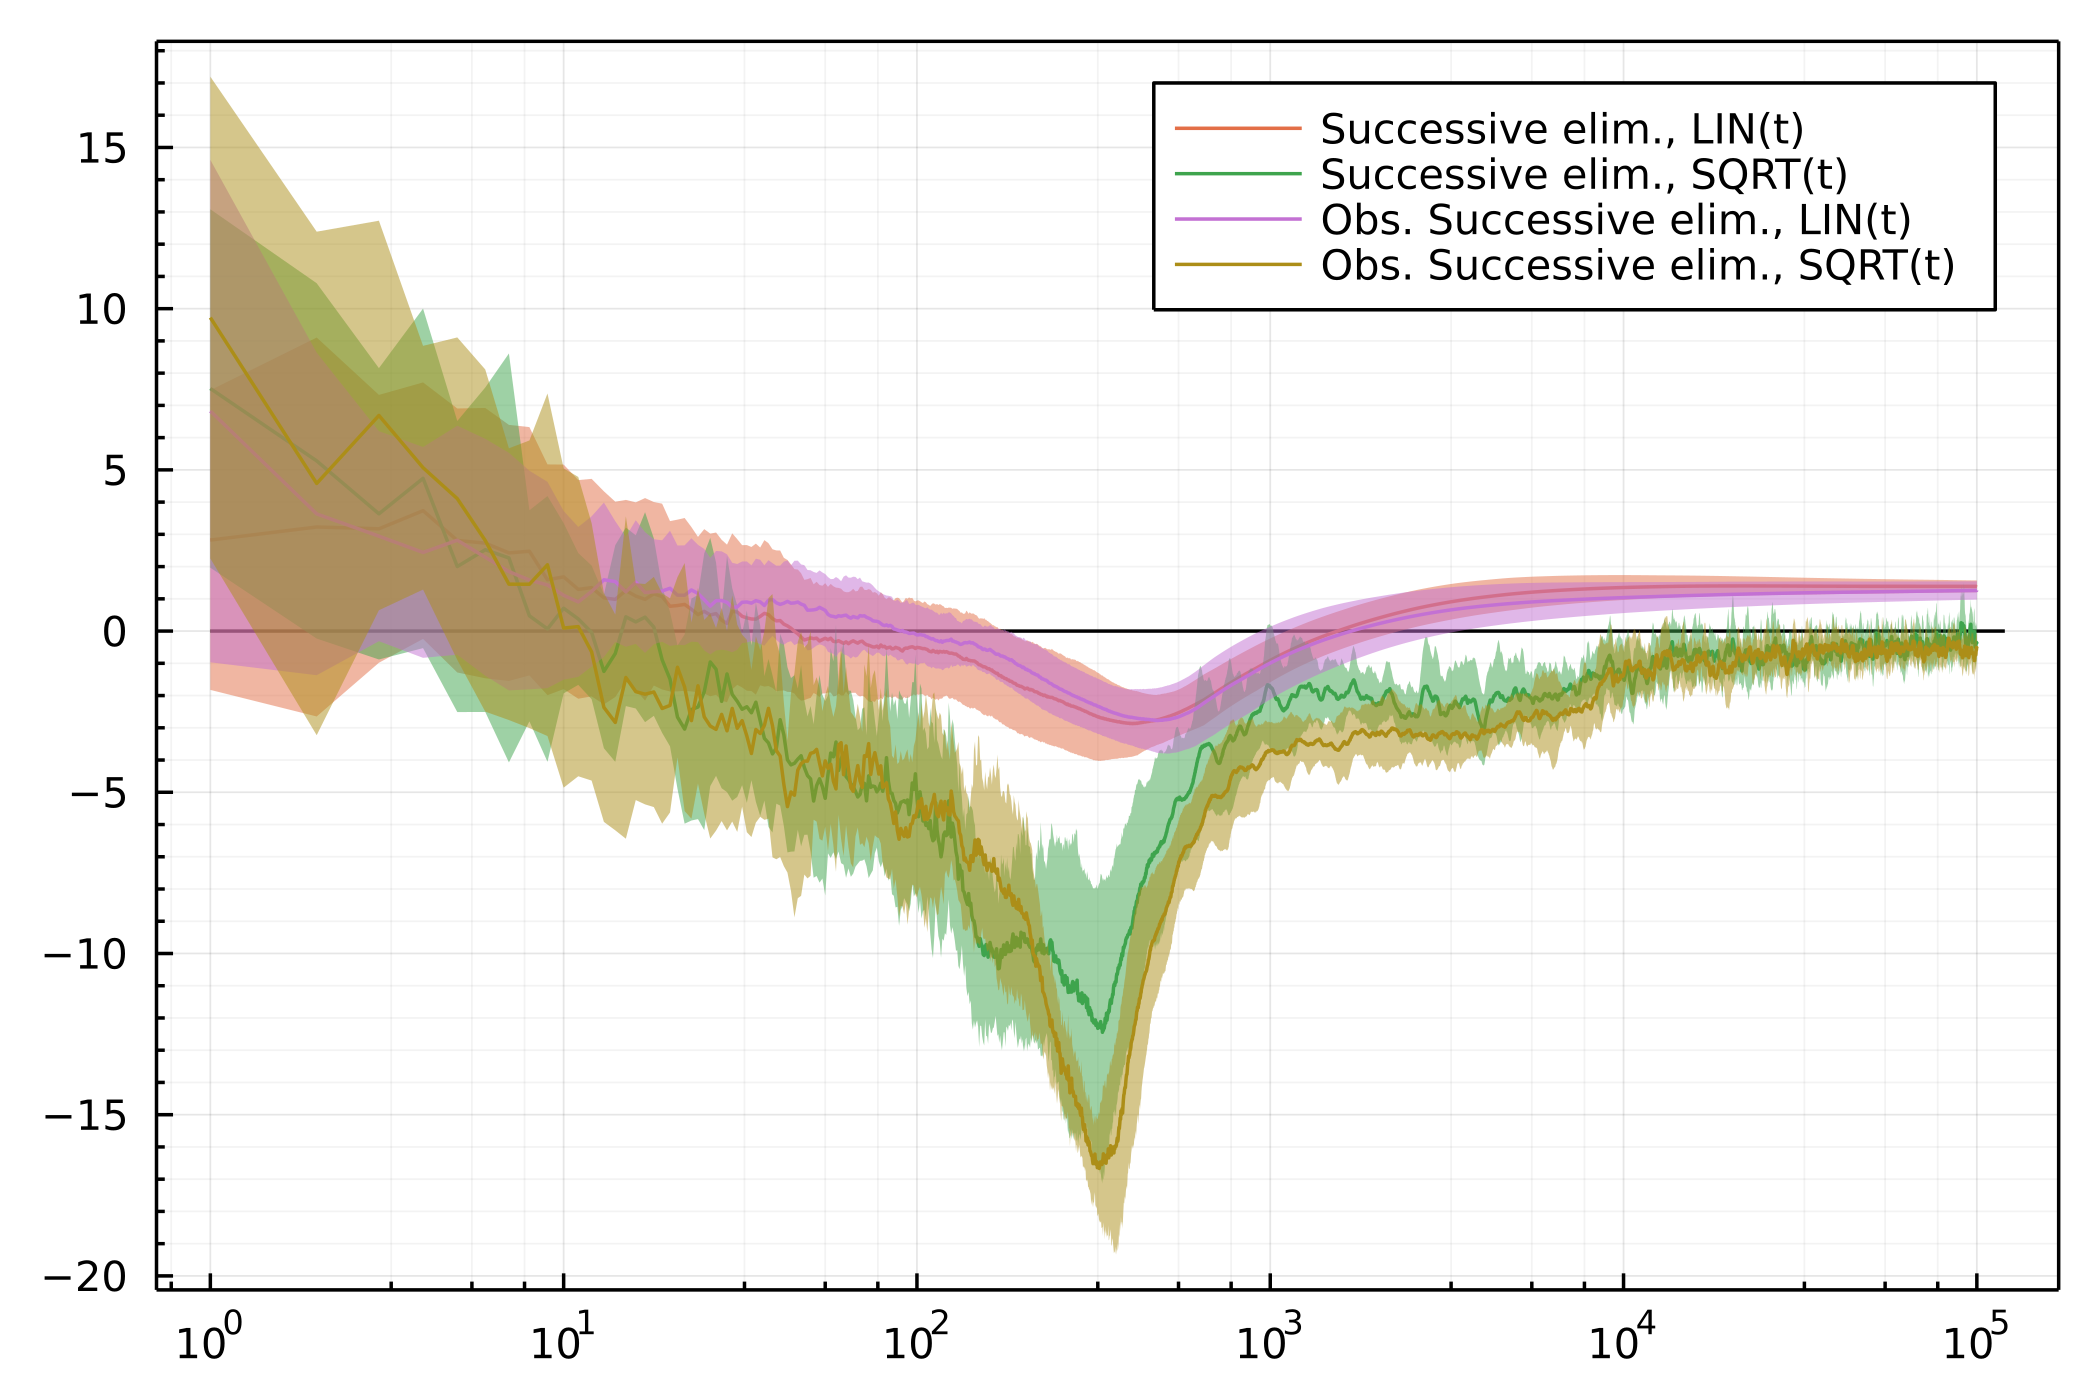
\includegraphics[width=0.8\textwidth]{sg/succ/tag_3_02_SuccessiveElimination_ObservableSuccessiveElimination_LinT_SqrtT_2_6.png}
    \caption[Convergence of the family of Successive elimination algorithms on a state with mixed optimal strategies]{
        The graph displays dependence of the deviation of the learned values from the true values on iteration step $t$ on an instance \tagname{3}{02} in a state $s = \left(2, 6\right)$, where a mixed strategy is optimal.
        The two step functions are included in the comparison.
    }
    \label{apx:sgexp:succ:fig:tag302:26}
\end{figure}
In this state of \tagname{3}{02} \reffig{exp:sg:games:tag:examples:32}, the mixed strategy initially contained actions which was not in the optimal strategy and thus the graph of the value iteration dips below the optimal value.
After the wrong action is not used any more, the value approaches the optimal zero deviation.
Moreover, the $\sqrtt$ step converges much closer than the $\lint$ arithmetic average.
On the other hand, it again fluctuates much more aggressively.

The Successive elimination bandit improves over the $\epsilon$-greedy in randomized decisions, but as well as Best of N, it can degrade to pure strategy by deactivating a wrong arm.
This could be prevented by tuning the $\alpha$ parameter for a specific problem.
Here, the $\sqrtt$ method can be beneficial, but can also lead to larger deviation when combined with the another problem mentioned first.

\section{UCB}\label{apx:sgexp:ucb}
The Upper Confidence Bound bandit algorithm is an alternation of the Successive elimination bandit.
In contrast, it does not deactivate presumably bad arms, but it always optimistically selects the best arm.
Even though it performs well in learning MDPs, it is primarily designed to converge to the single best action, i.e. pure strategy.
In these experiments, the search parameter is $\alpha = 20$.
Now, we analyse it on stochastic games together with its observable variant.

The first comparison is done on the \tagname{3}{01} and \tagname{3}{02} instances and is depicted in figure \reffig{apx:sgexp:ucb:fig:tags}.
\begin{figure}[ht]
    \begin{subfigure}[t]{0.45\linewidth}
        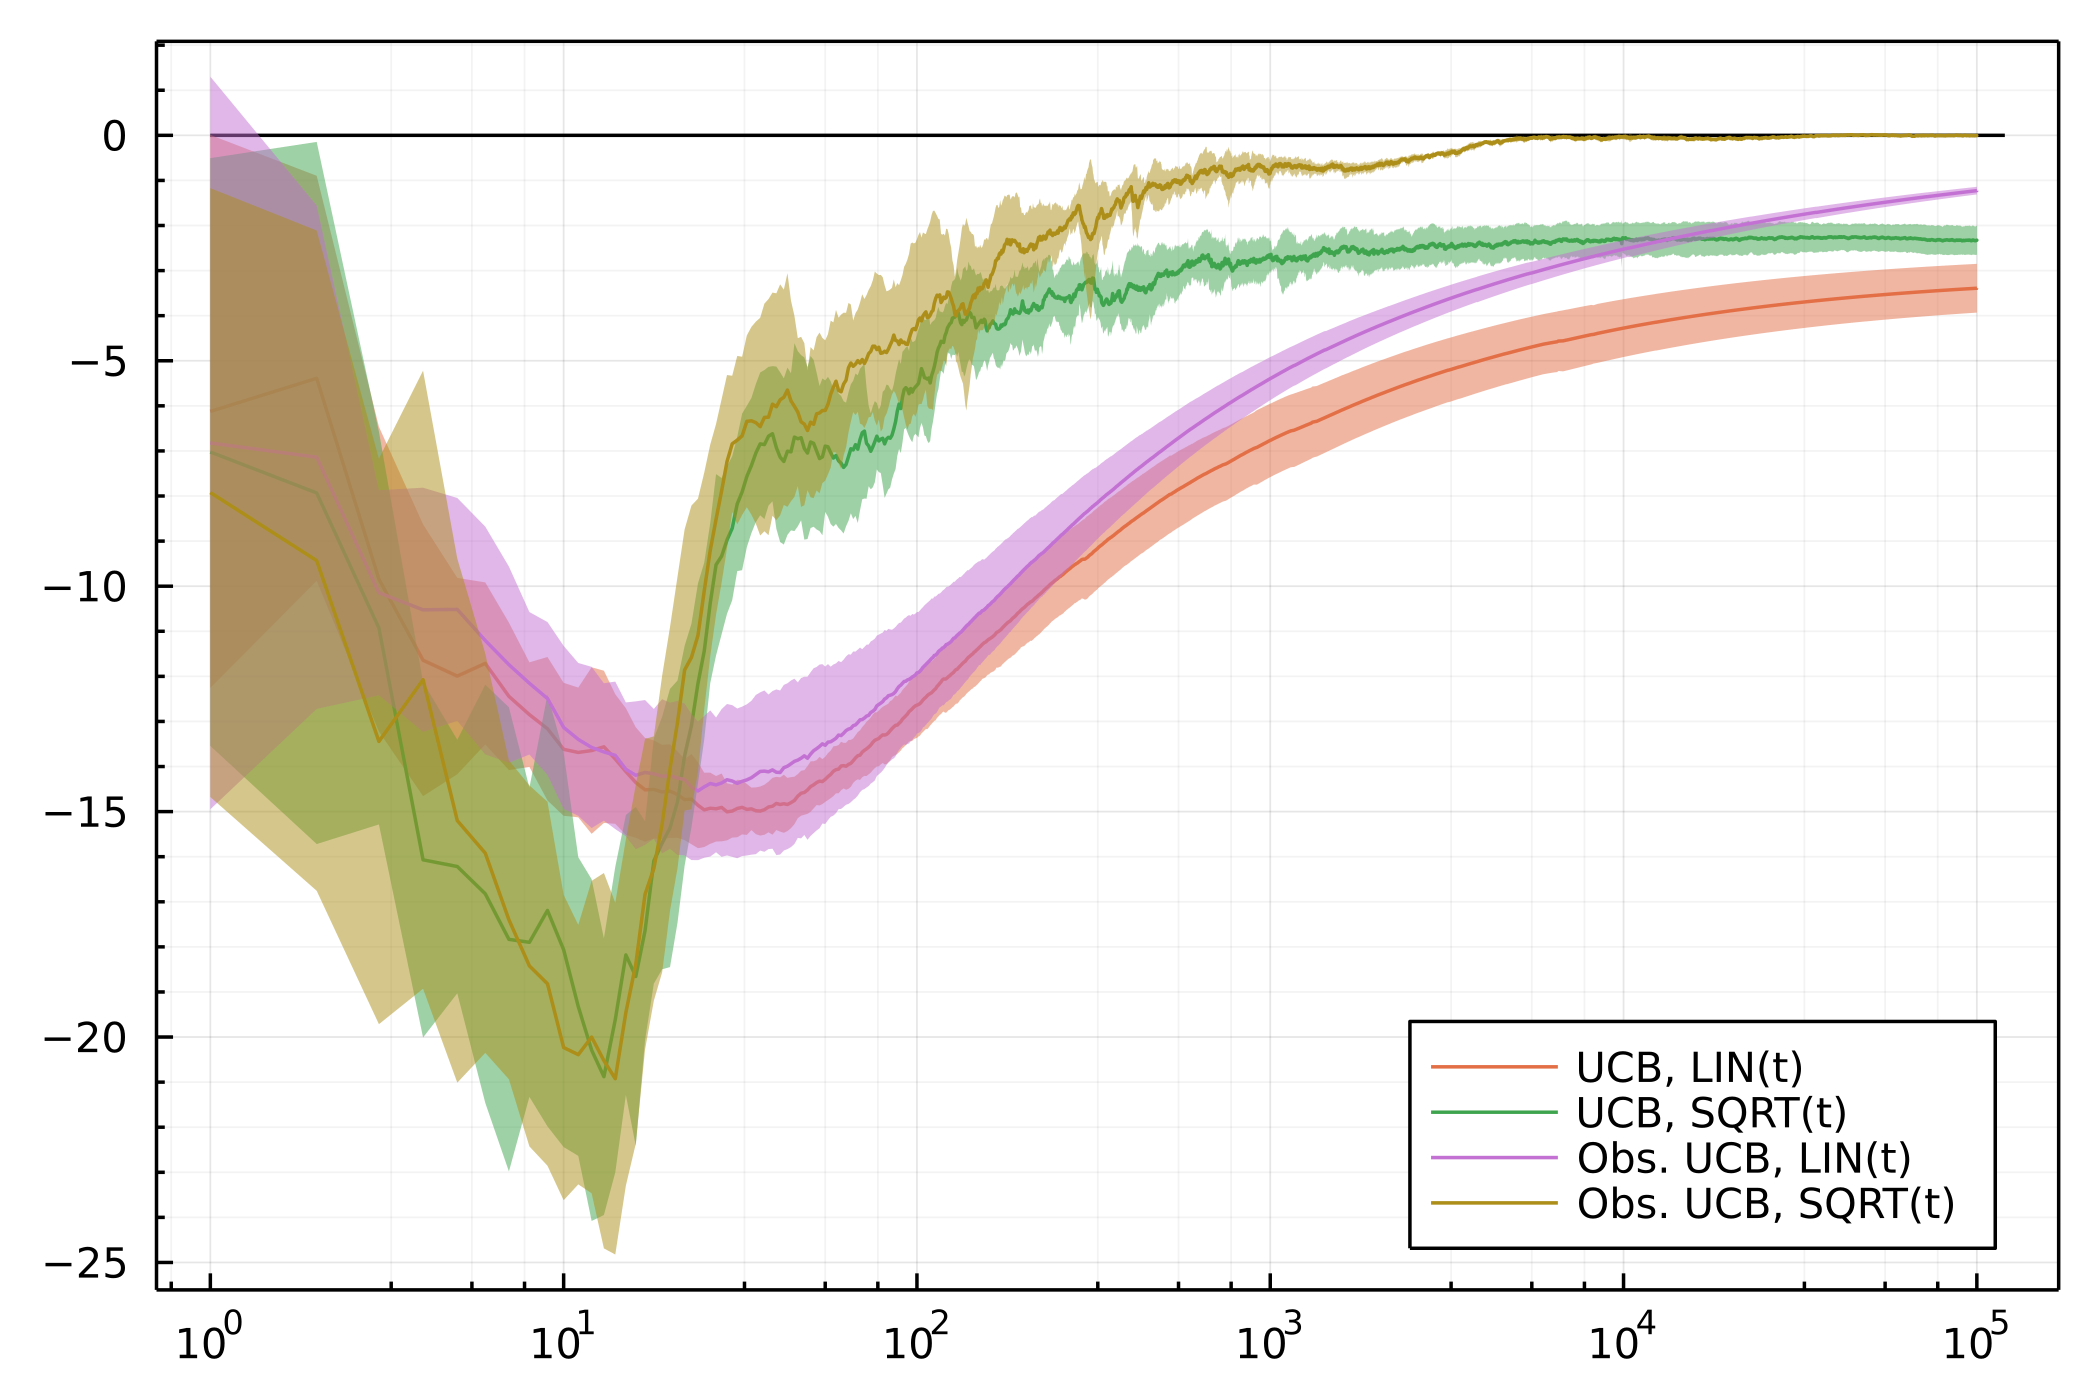
\includegraphics[width=1\textwidth]{sg/ucb/tag_3_01_UCB_ObservableUCB_LinT_SqrtT_2_4.png}
        \caption{\tagname{3}{01} in a state $s = \left(2, 4\right)$}
        \label{apx:sgexp:succ:fig:tag301:24}
    \end{subfigure}
    \hfill
    \begin{subfigure}[t]{0.45\linewidth}
        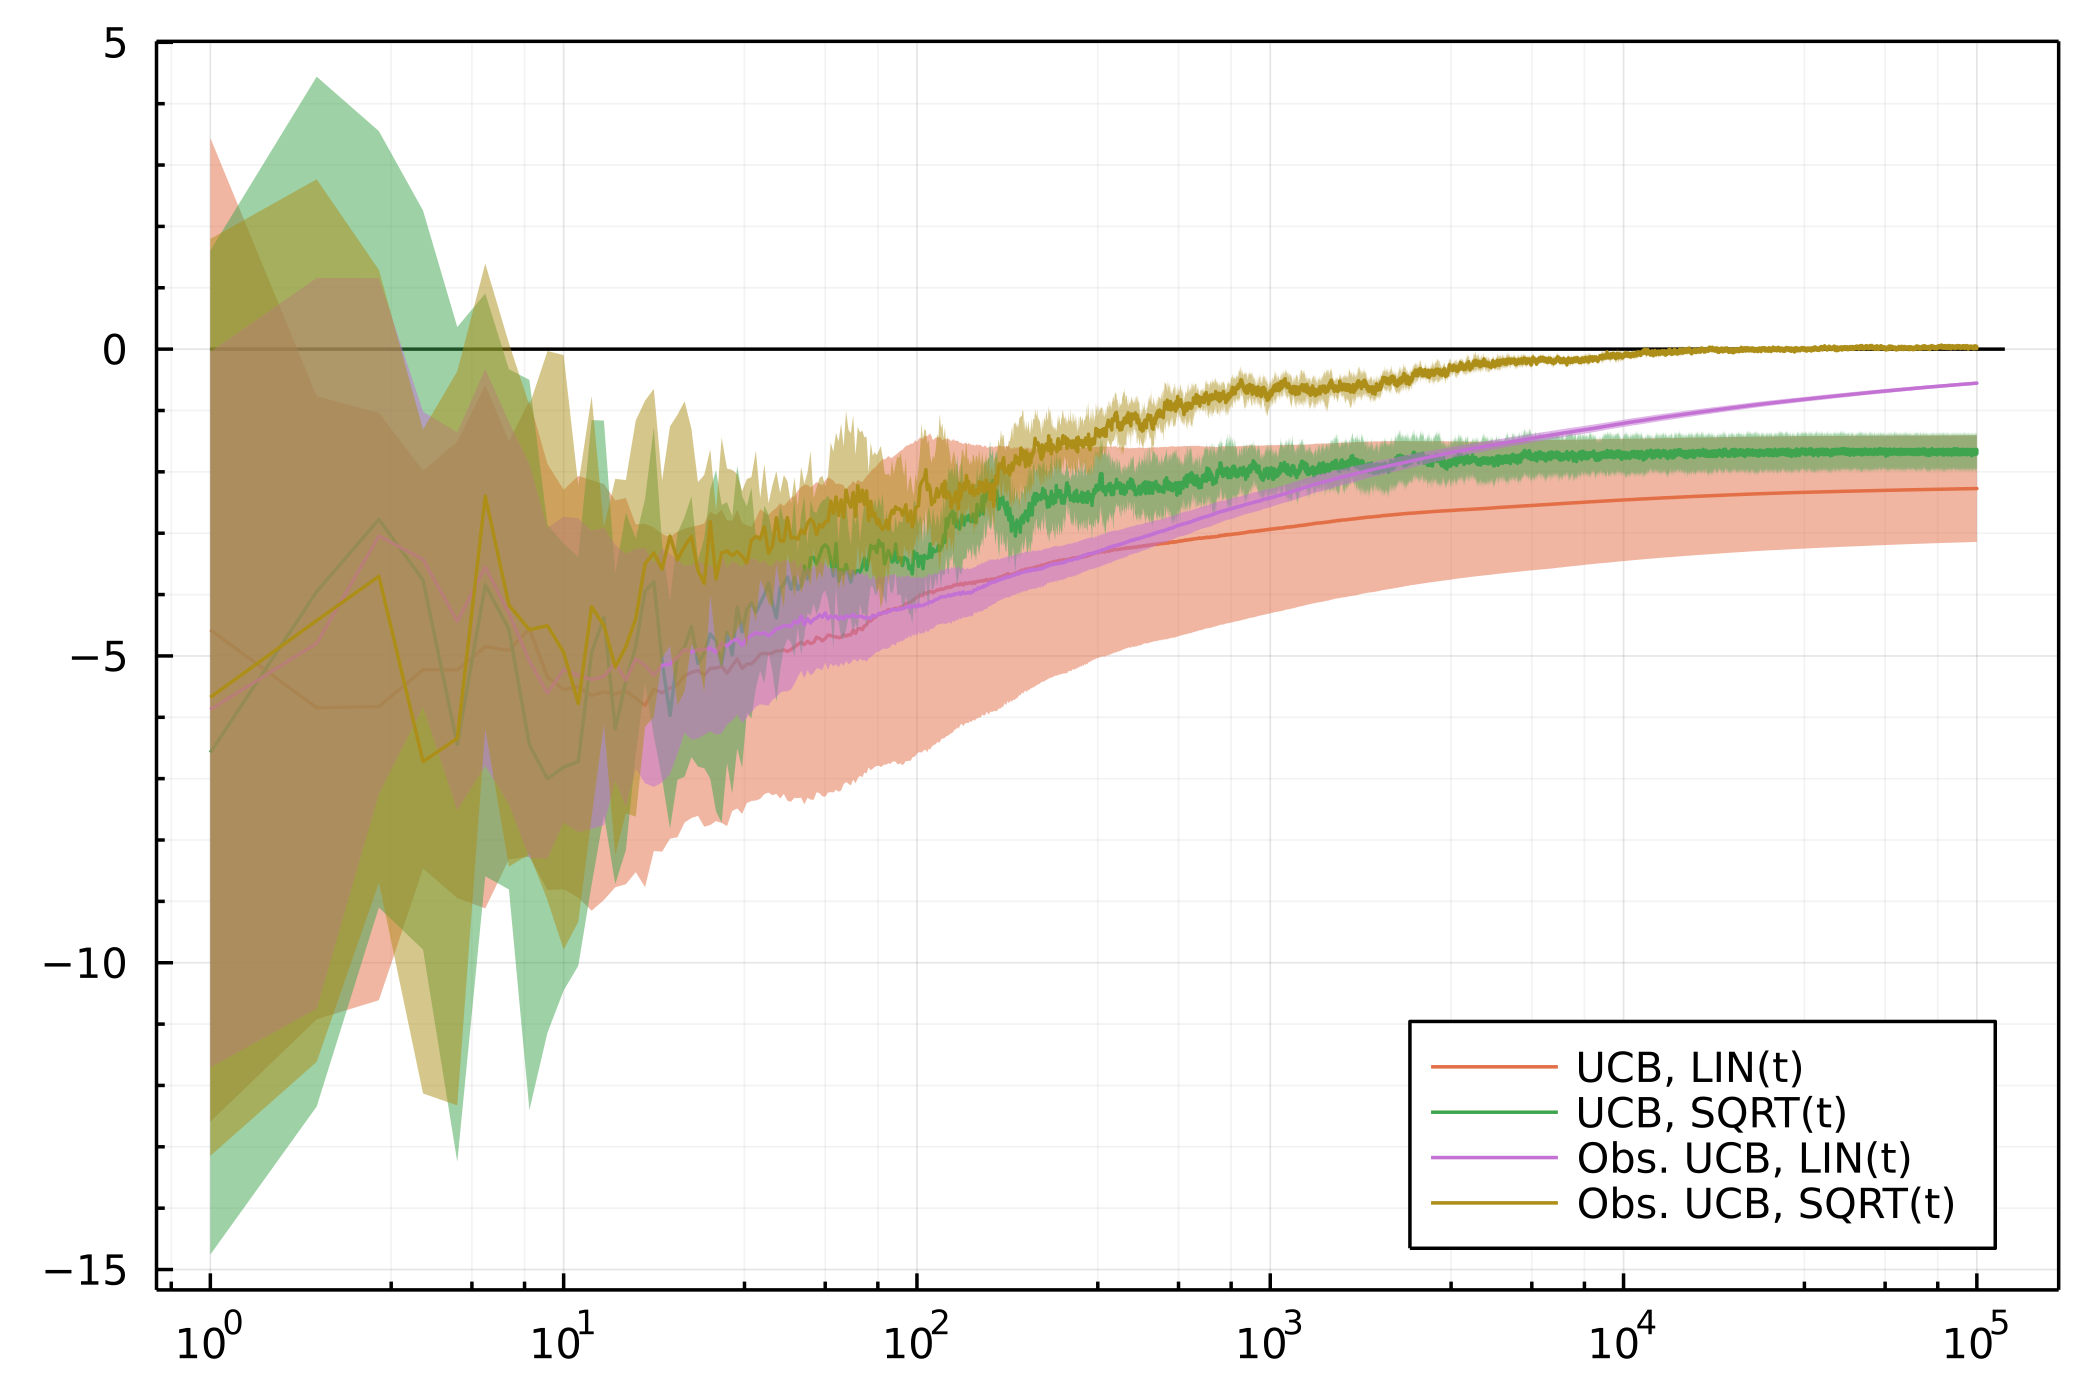
\includegraphics[width=1\textwidth]{sg/ucb/tag_3_01_UCB_ObservableUCB_LinT_SqrtT_3_3.png}
        \caption{\tagname{3}{01} in a state $s = \left(3, 3\right)$}
        \label{apx:sgexp:succ:fig:tag301:33}
    \end{subfigure}
    \begin{subfigure}[t]{0.45\linewidth}
        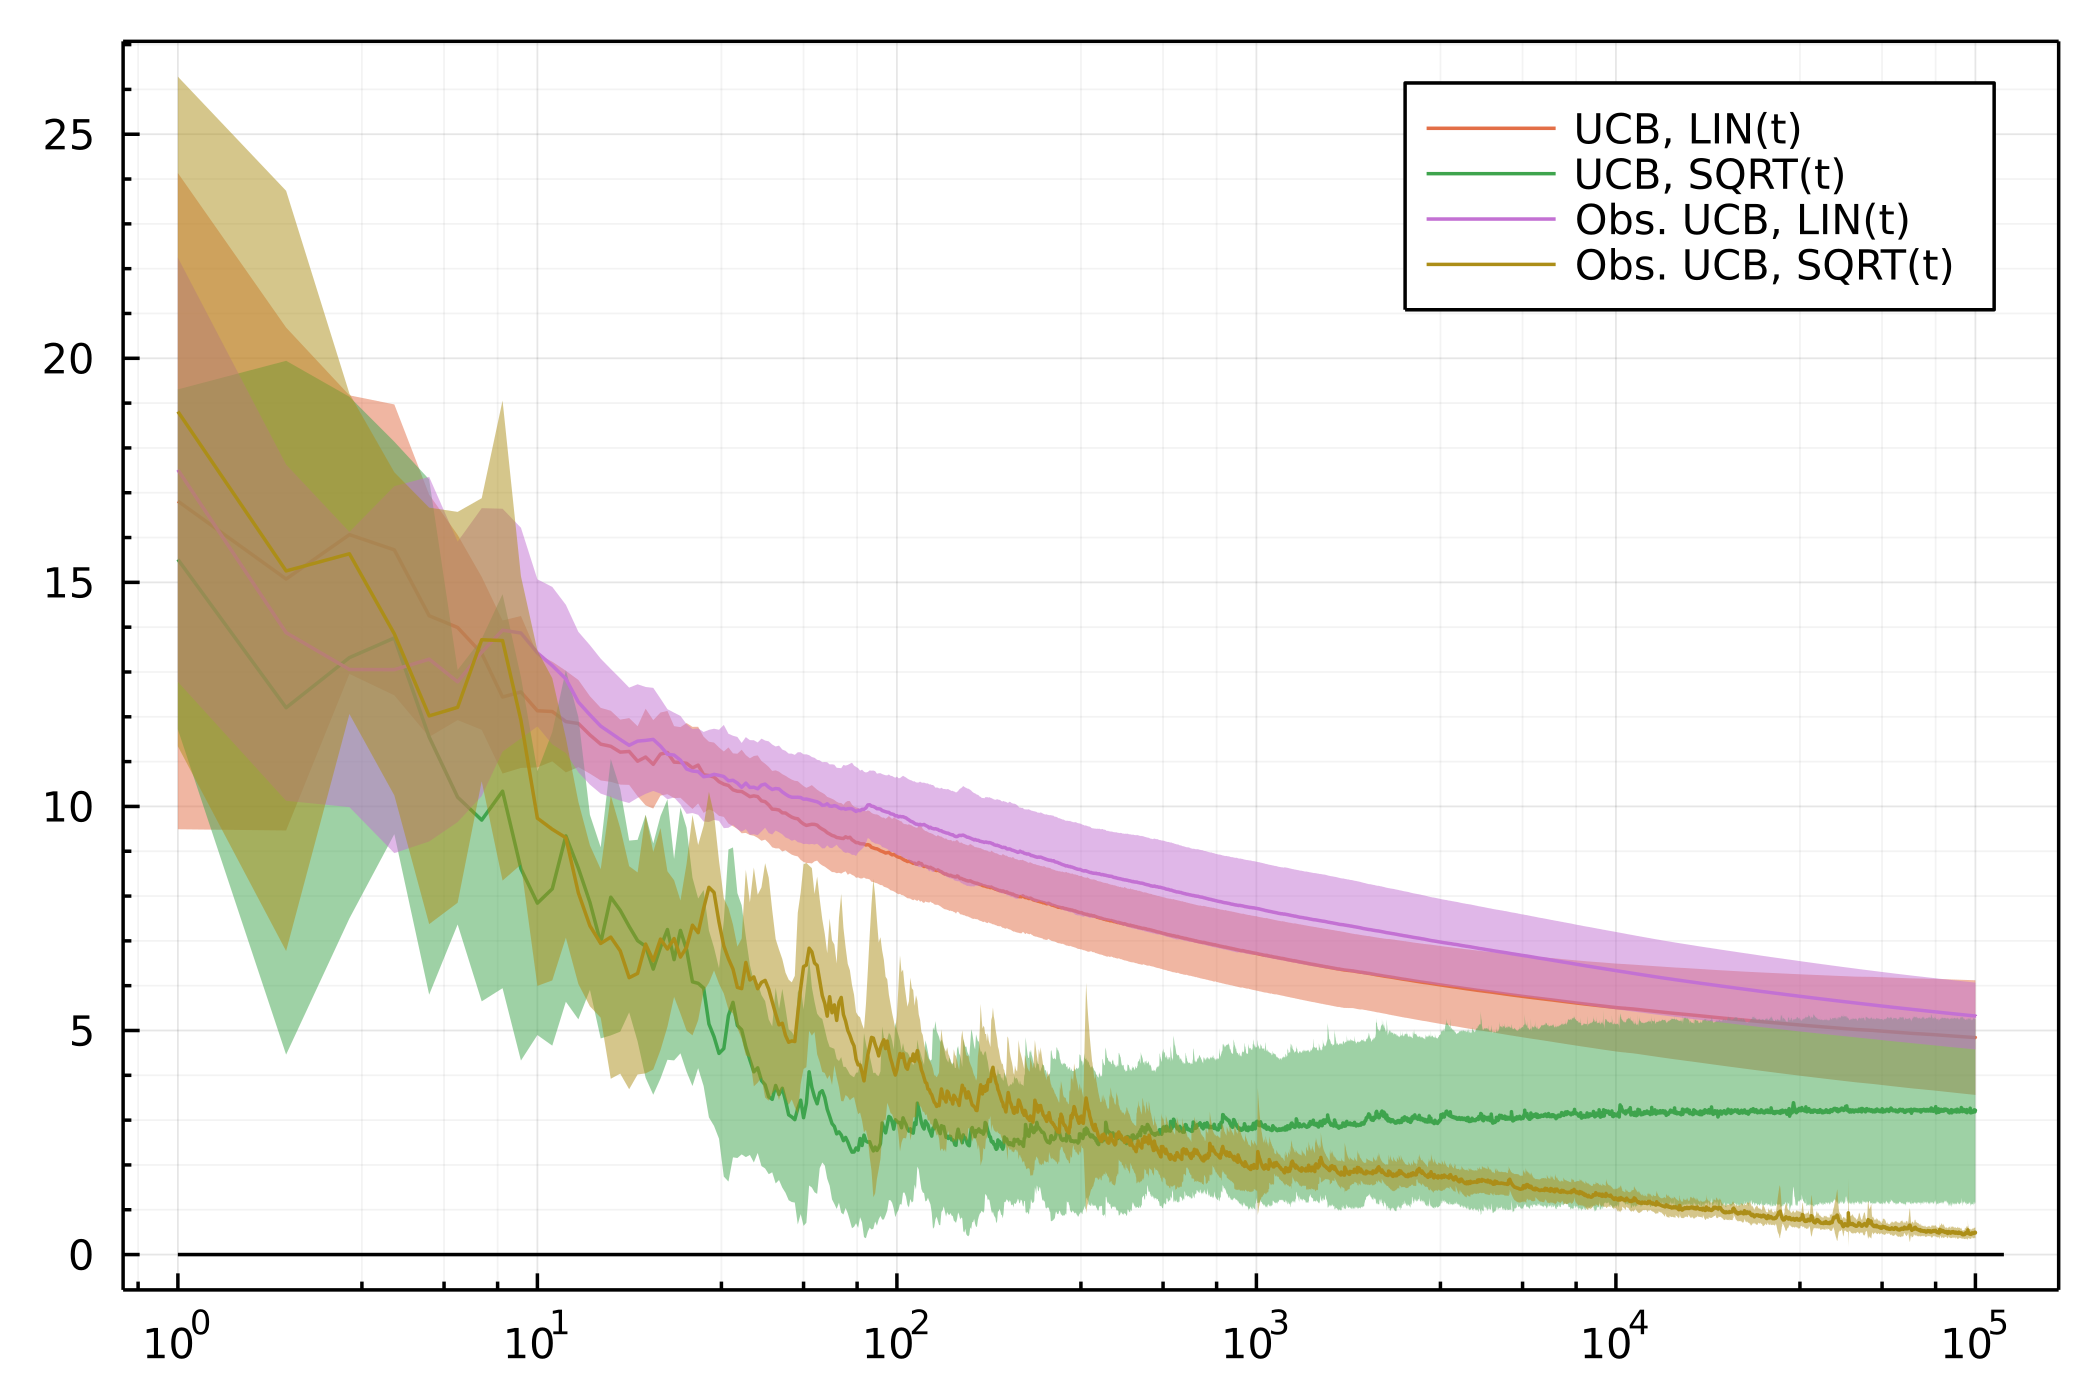
\includegraphics[width=1\textwidth]{sg/ucb/tag_3_02_UCB_ObservableUCB_LinT_SqrtT_2_4.png}
        \caption{\tagname{3}{02} in a state $s = \left(2, 4\right)$}
        \label{apx:sgexp:succ:fig:tag302:24}
    \end{subfigure}
    \hfill
    \begin{subfigure}[t]{0.45\linewidth}
        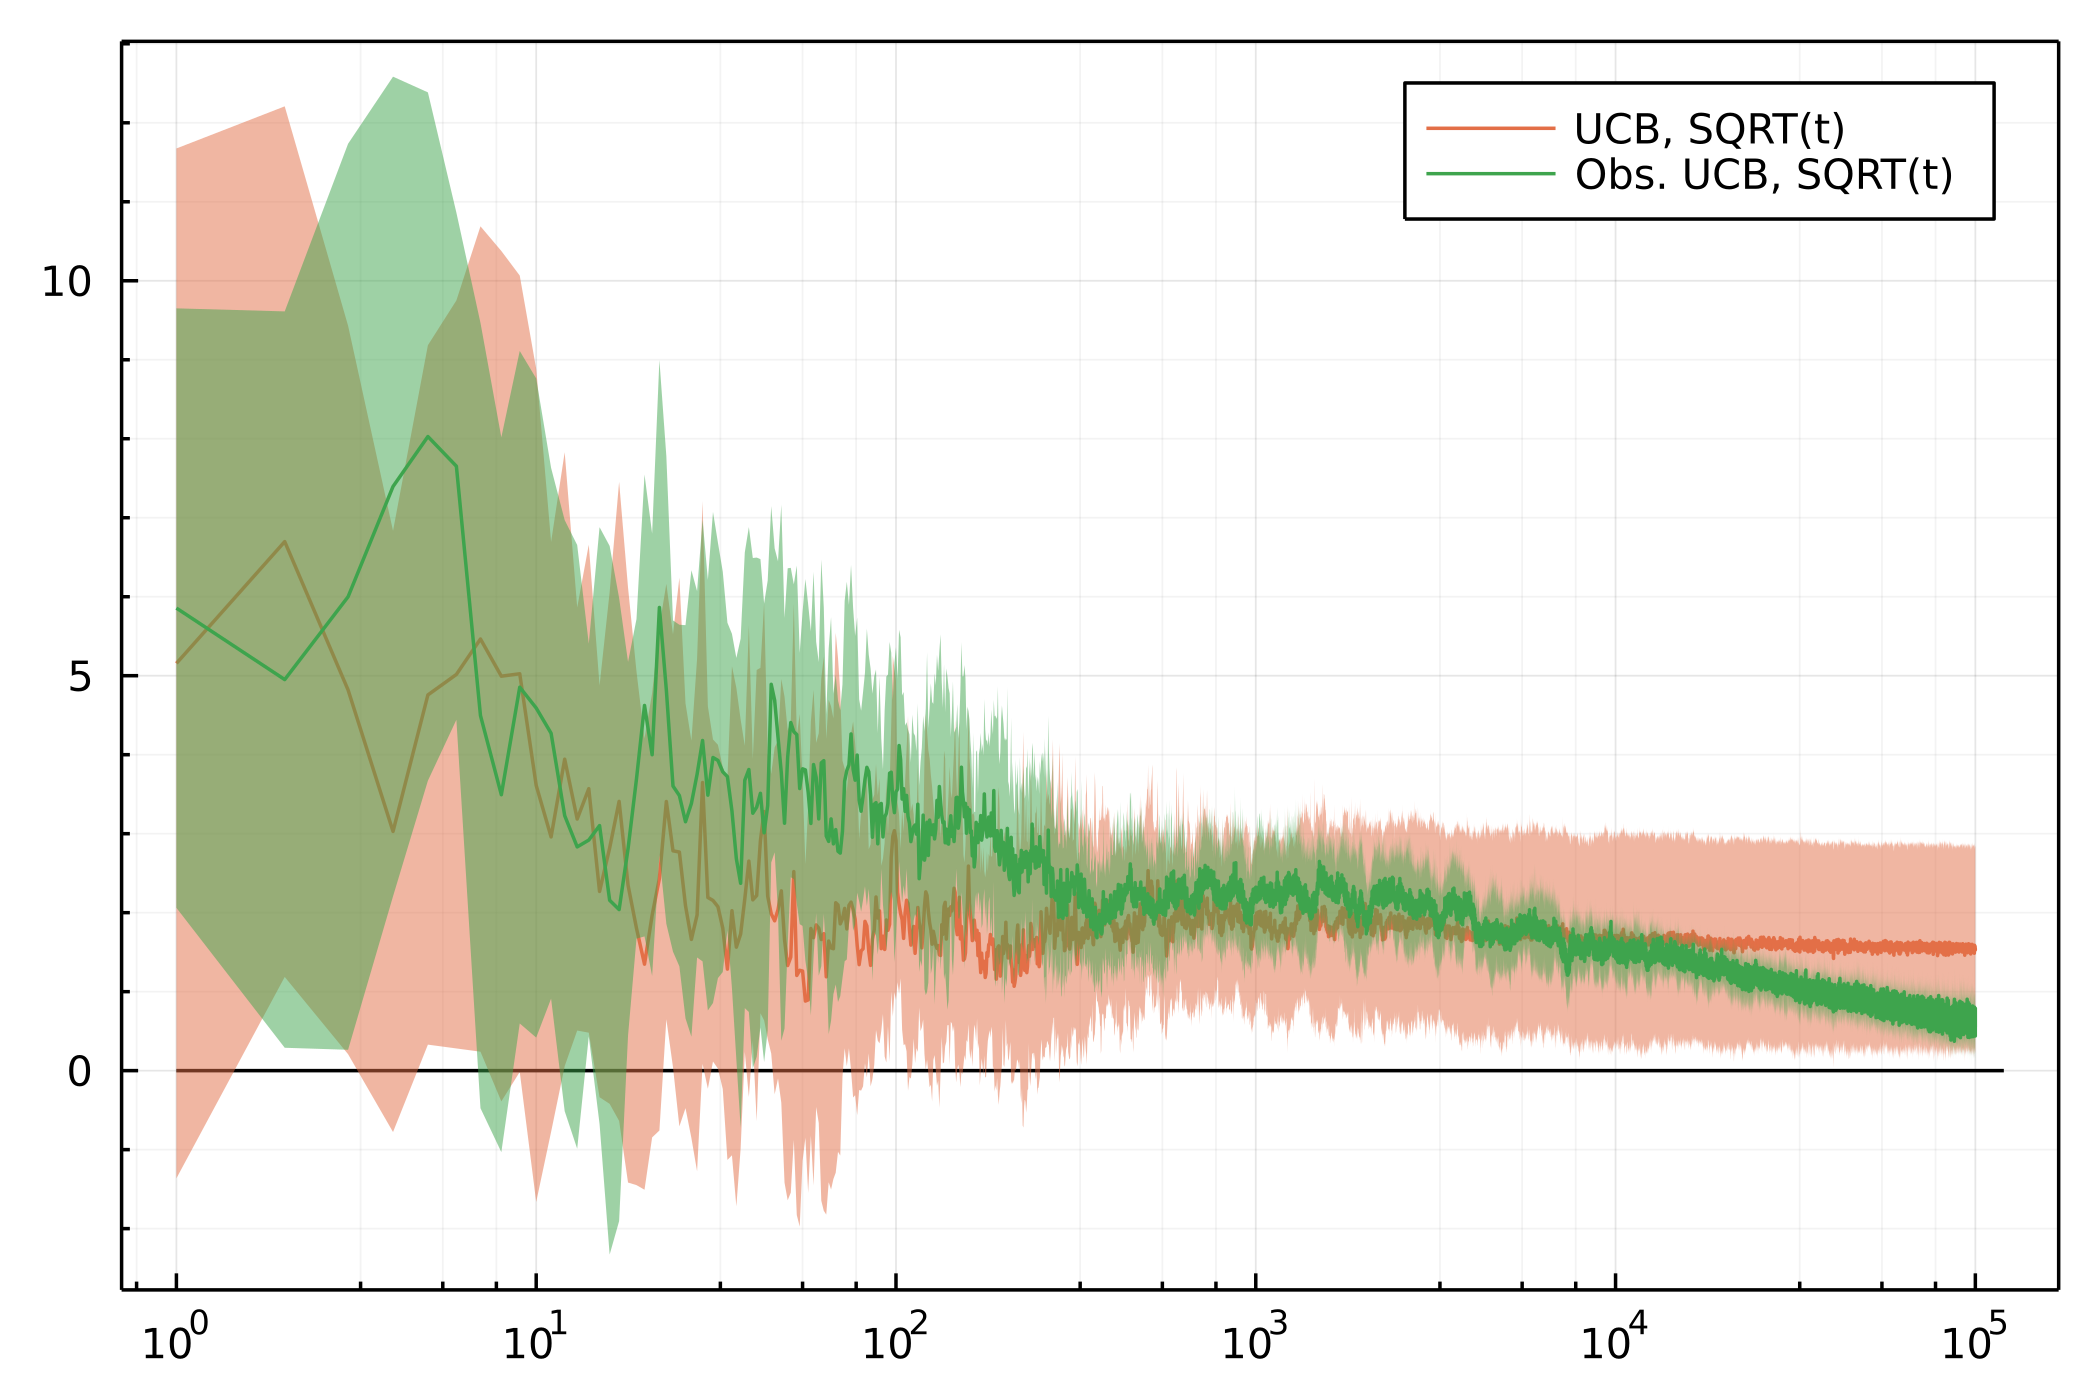
\includegraphics[width=1\textwidth]{sg/ucb/tag_3_02_UCB_ObservableUCB_SqrtT_4_4.png}
        \caption{\tagname{3}{02} in a state $s = \left(4, 4\right)$}
        \label{apx:sgexp:succ:fig:tag302:44}
    \end{subfigure}
    \caption[Comparison of observable and non-observable UCB multi-armed bandits on mixed-strategy states]{
        The graphs display convergence of observable and standard UCB multi-armed bandits with both of the step functions, $\lint$ and $\sqrtt$, and the development of learned values change in time represented by discrete iteration steps.
        The comparison is done on two instances, \tagname{3}{01} and \tagname{3}{02}, in states where true optimal strategies are mixed.
    }
    \label{apx:sgexp:ucb:fig:tags}
\end{figure}
Here are shown two hard states from every chosen instance, which were either hard for previous bandits or they did not converge close to the optimum.
From these graphs, it can be derived that the observable variant of UCB is significantly better than the non-observable UCB.
In all these states, it either finds the optimum or continues pushing the deviation to 0 even after the standard algorithm finds its best pure strategy and converges to some suboptimal value.

Also, in the case of UCB, the $\sqrtt$ accumulation step boosts the speed of convergence for both of the algorithms without unnecessary fluctuations as it was with previous bandits.
Even though the observable UCB with $\lint$ step appears to approach 0 as well, the $\sqrtt$ reaches this value much faster and most importantly stays there as opposed to other multi-armed bandits.

Here is another example of the same phenomenon as described above, but this time for a \chasename{5} instance \reffig{exp:sg:games:chase:examples:5}.
\begin{figure}[ht]
    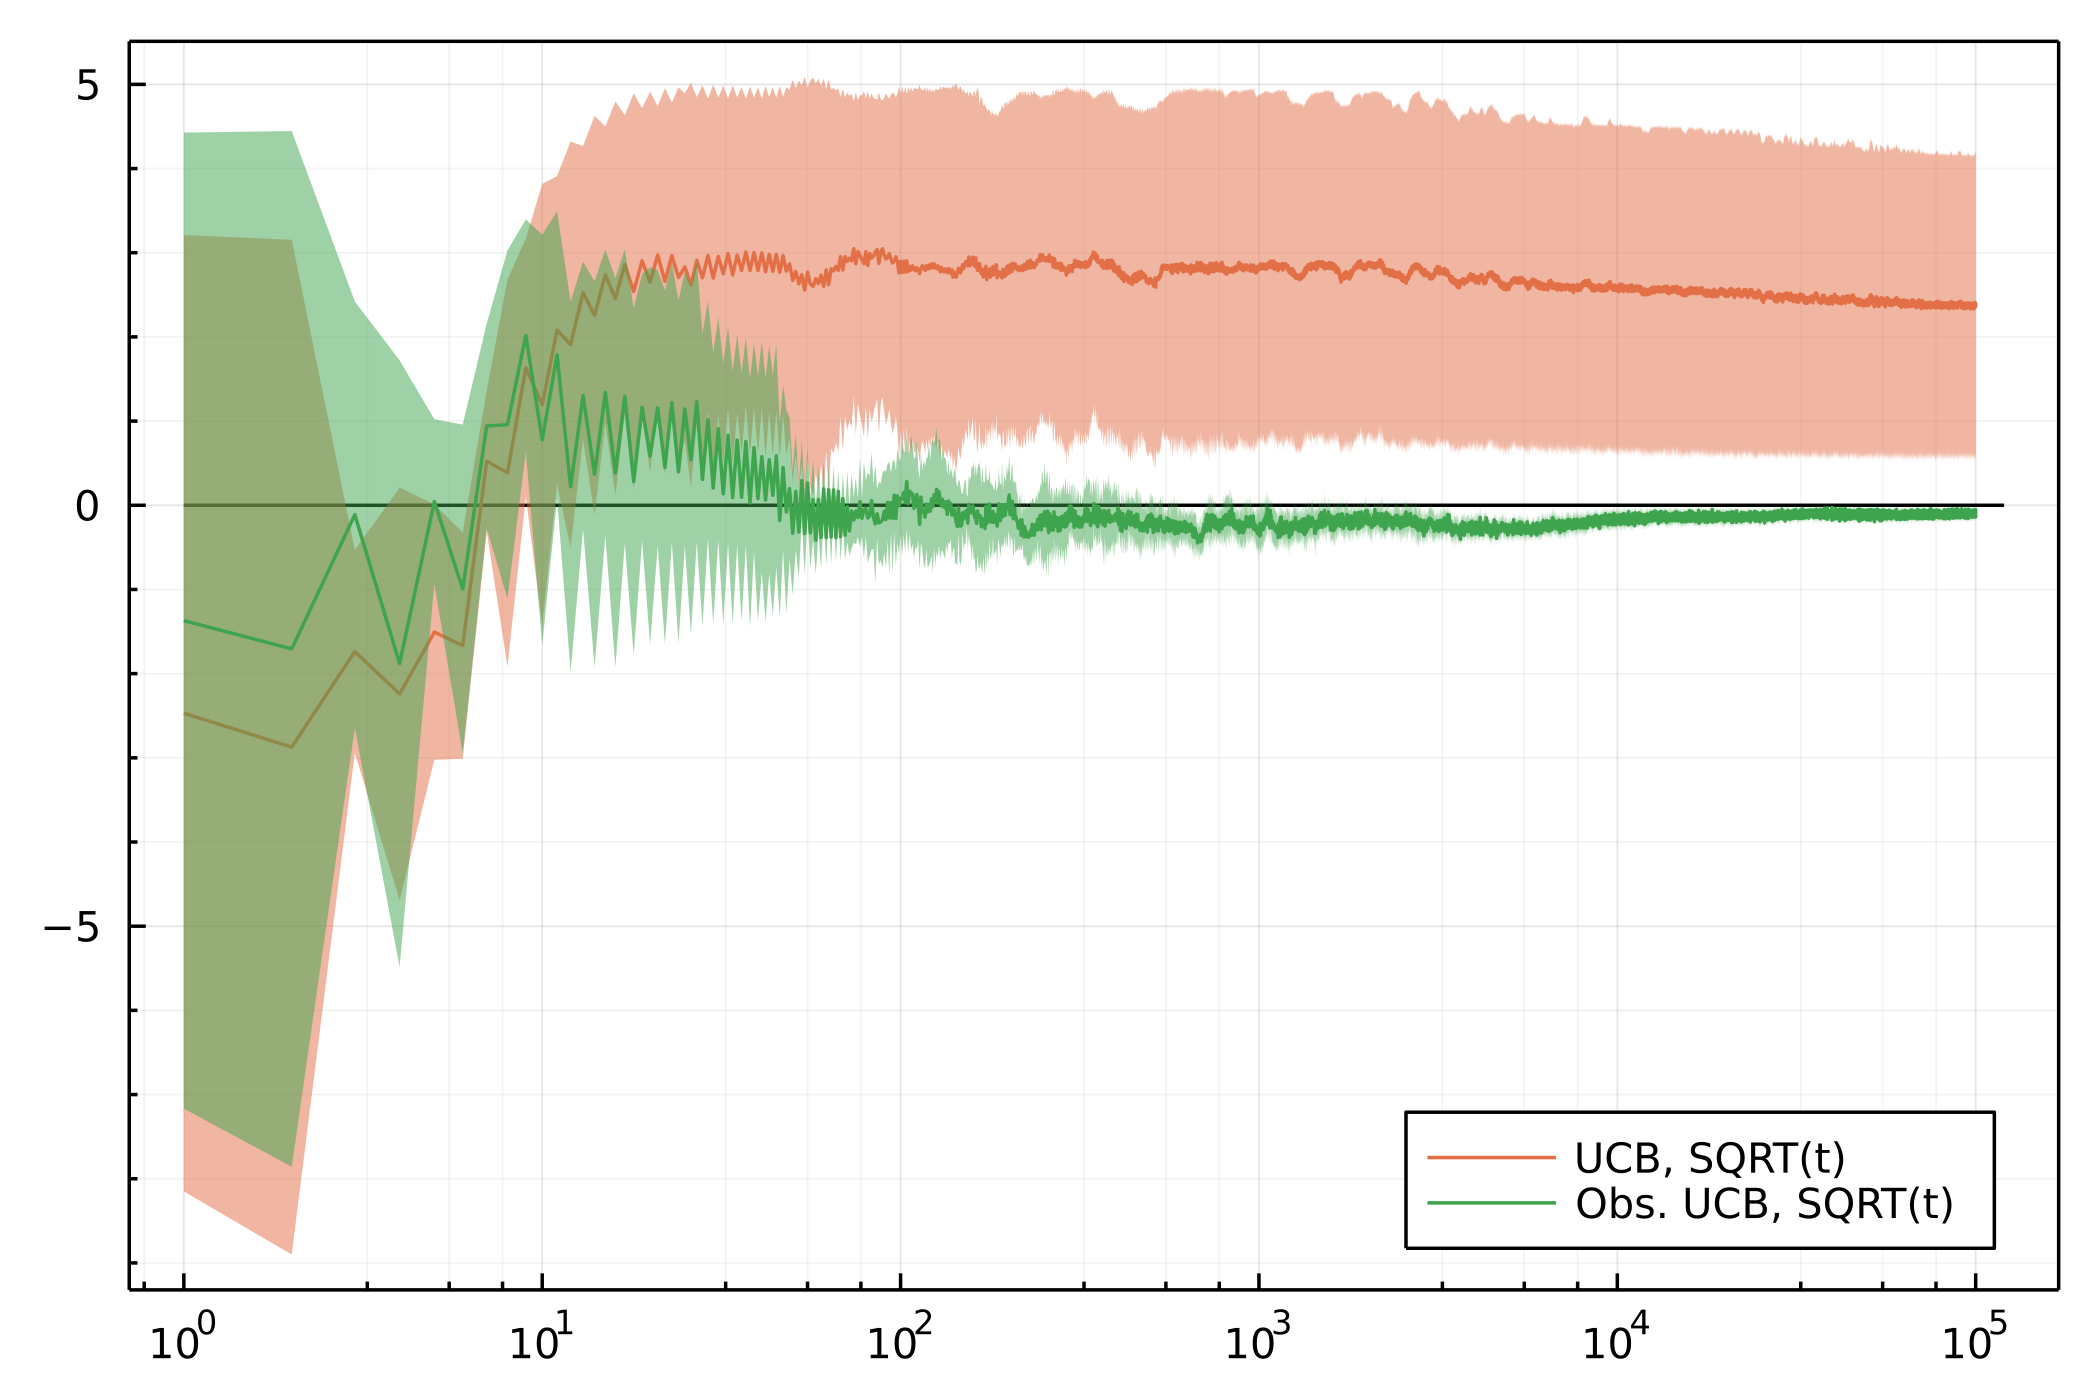
\includegraphics[width=0.8\textwidth]{sg/ucb/graphs_5_01_UCB_ObservableUCB_SqrtT_3_3.png}
    \caption[Comparison of observable and unobservable UCB on a \chasename{5} instance]{
        This comparison chart depict performance of UCB in comparison to its observable counterpart on a \textbf{Chase} instance \chasename{5} in a mixed-strategy state $s = \left(3, 3\right)$.
        The $y$ axis shows deviation from the ground truth represented by the black constant function depending on the time stamp $t$ on the $x$ axis.
    }
    \label{exp:sg:ucb:fig:unconvergence}
\end{figure}
This particular state is interesting, because both bandits start in the same vertex of the graph in \reffig{exp:sg:games:chase:examples:5}, this node being the node $3$.
The graph visualization implies that both players would have to randomize their action selection, i.e. employ a mixed strategy.
This is because if on of them committed to either using the loop and staying in the node $3$ or use action $2$ to reach vertex $5$, his adversary would instantly leverage this.
The runner would choose the opposite action, while the chaser would choose the same action.
From the graph, UCB has clearly an issue with converging in a mixed strategy state, while the average play variant tries to respond to the frequent choices by the adversary.

The observable UCB bandit converged to the optimal value in almost all states of all instances, or at least got very close.
In contrast, the standard UCB sometimes struggles to reach the optimum and finds the best pure strategy.
This showcases that the opponent's average play provides an actual advantage in bandit learning in stochastic games.
It permits the bandit originally intended to search for a single best action, to rather find the best response to the average play of its adversary.

Moreover, in this case the $\sqrtt$ step function is far superior to the $\lint$ and significantly improves the speed of convergence as is documented in the figures in this section.
Of all these combinations, the observable UCB bandit with the use of $\sqrtt$ dominated the other options.

\section{Exp3}\label{apx:sgexp:exp3}
The adversarial Exp3 bandit, in contrast to the others, was designed to learn a whole strategy rather than a single best action.

In figure \reffig{apx:sgexp:exp3:fig} are showcased 4 different examples of states with various difficulty.
\begin{figure}[ht]
    \begin{subfigure}[t]{0.45\linewidth}
        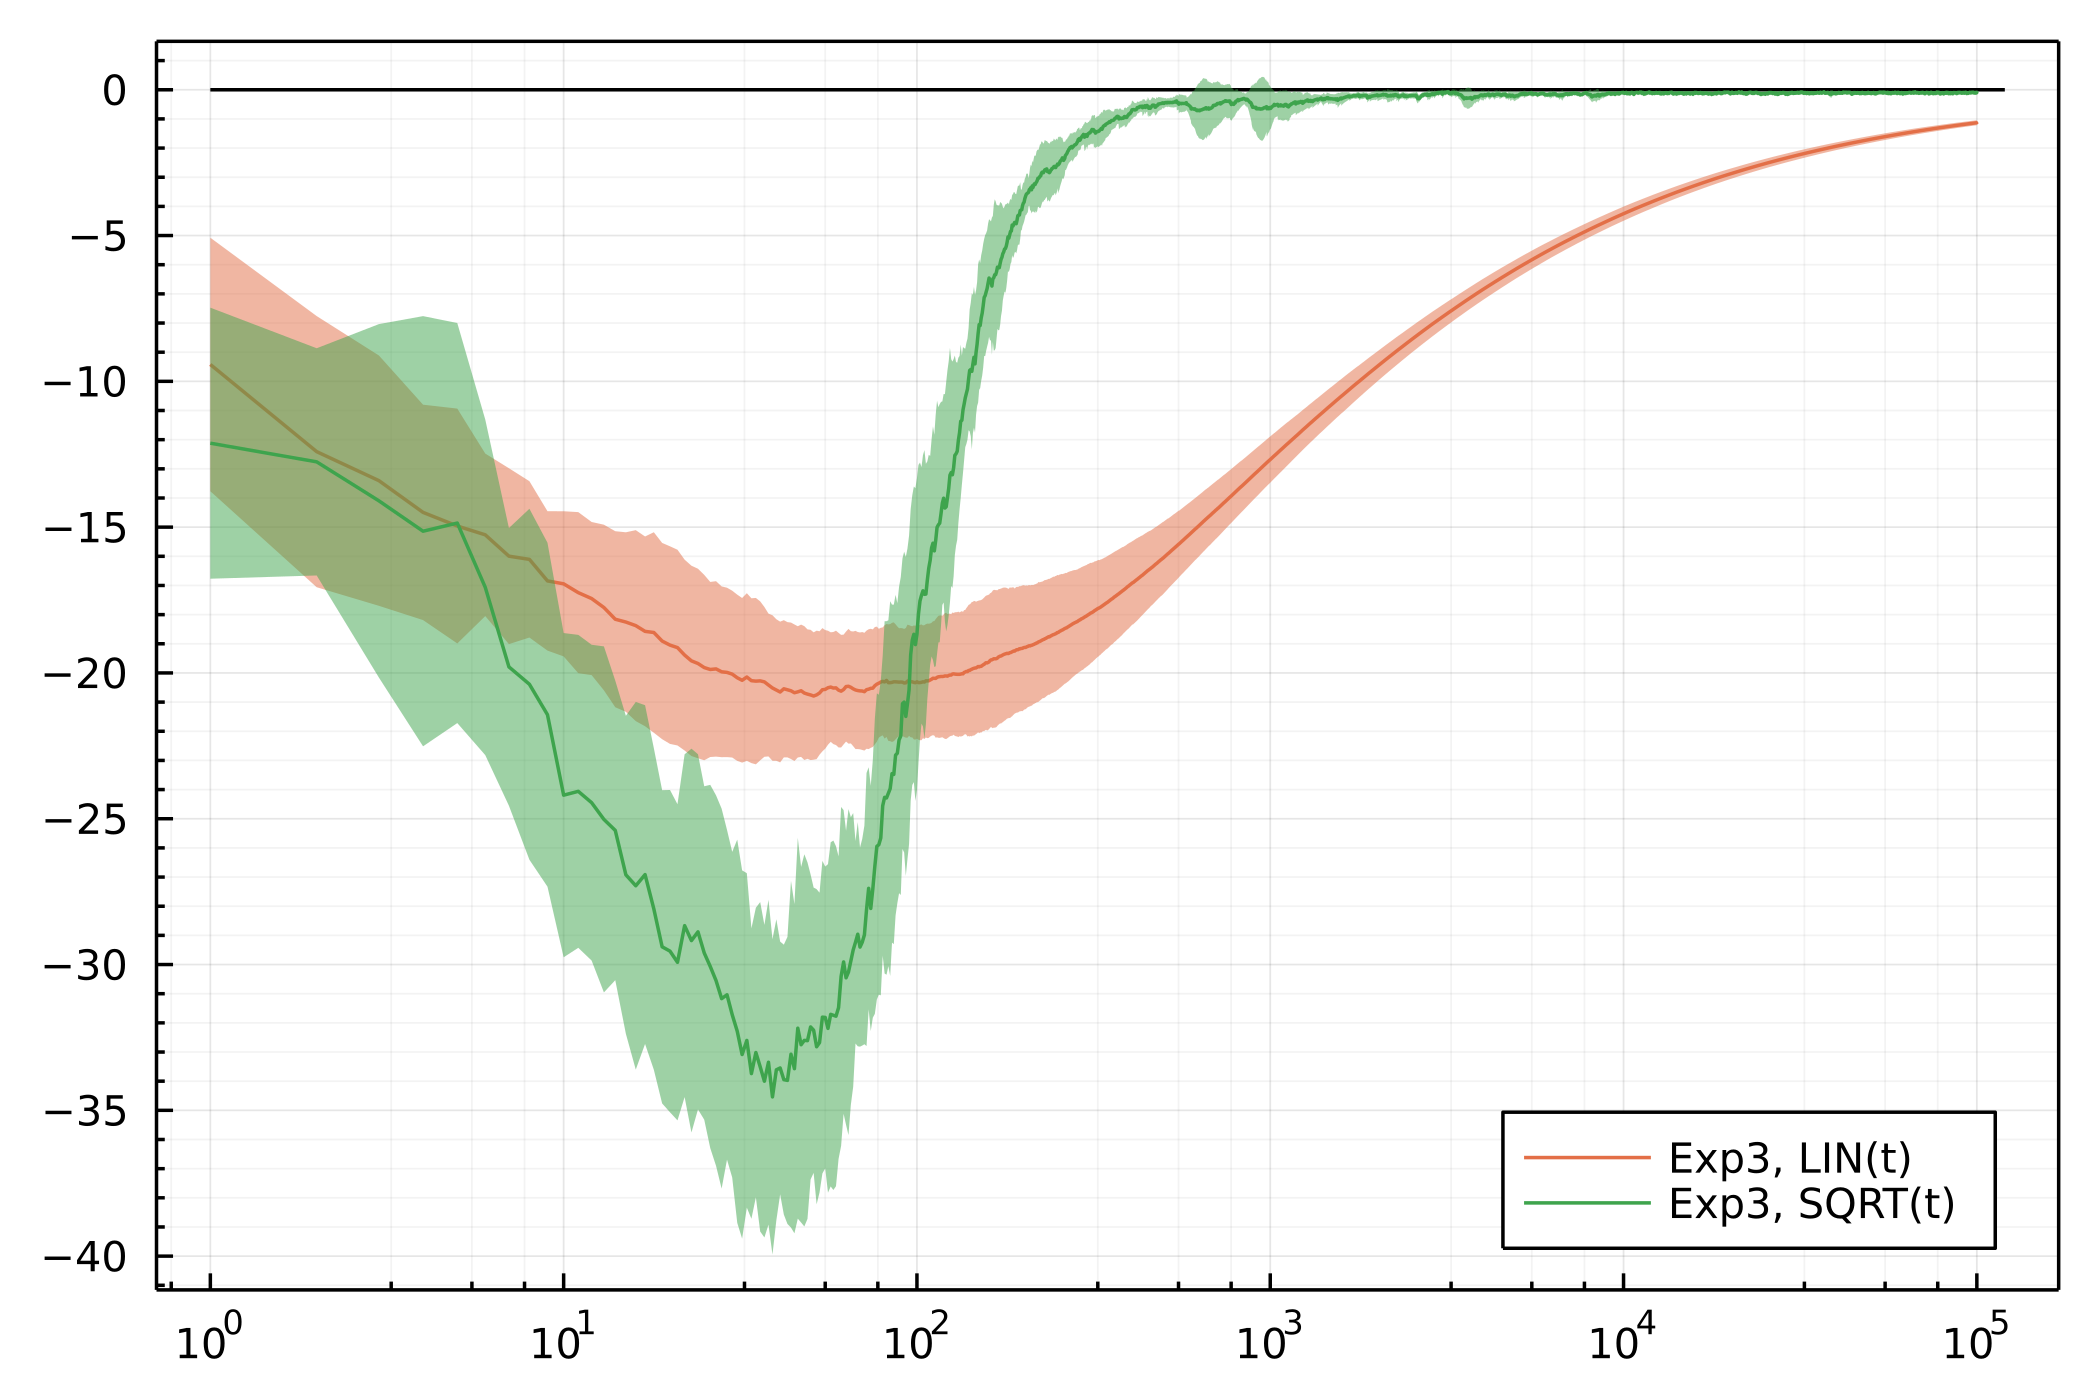
\includegraphics[width=1\textwidth]{sg/exp3/tag_3_01_Exp3_LinT_SqrtT_2_7.png}
        \caption{\tagname{3}{01} in a state $s = \left(2, 7\right)$}
        \label{apx:sgexp:exp3:fig:tag301:27}
    \end{subfigure}
    \hfill
    \begin{subfigure}[t]{0.45\linewidth}
        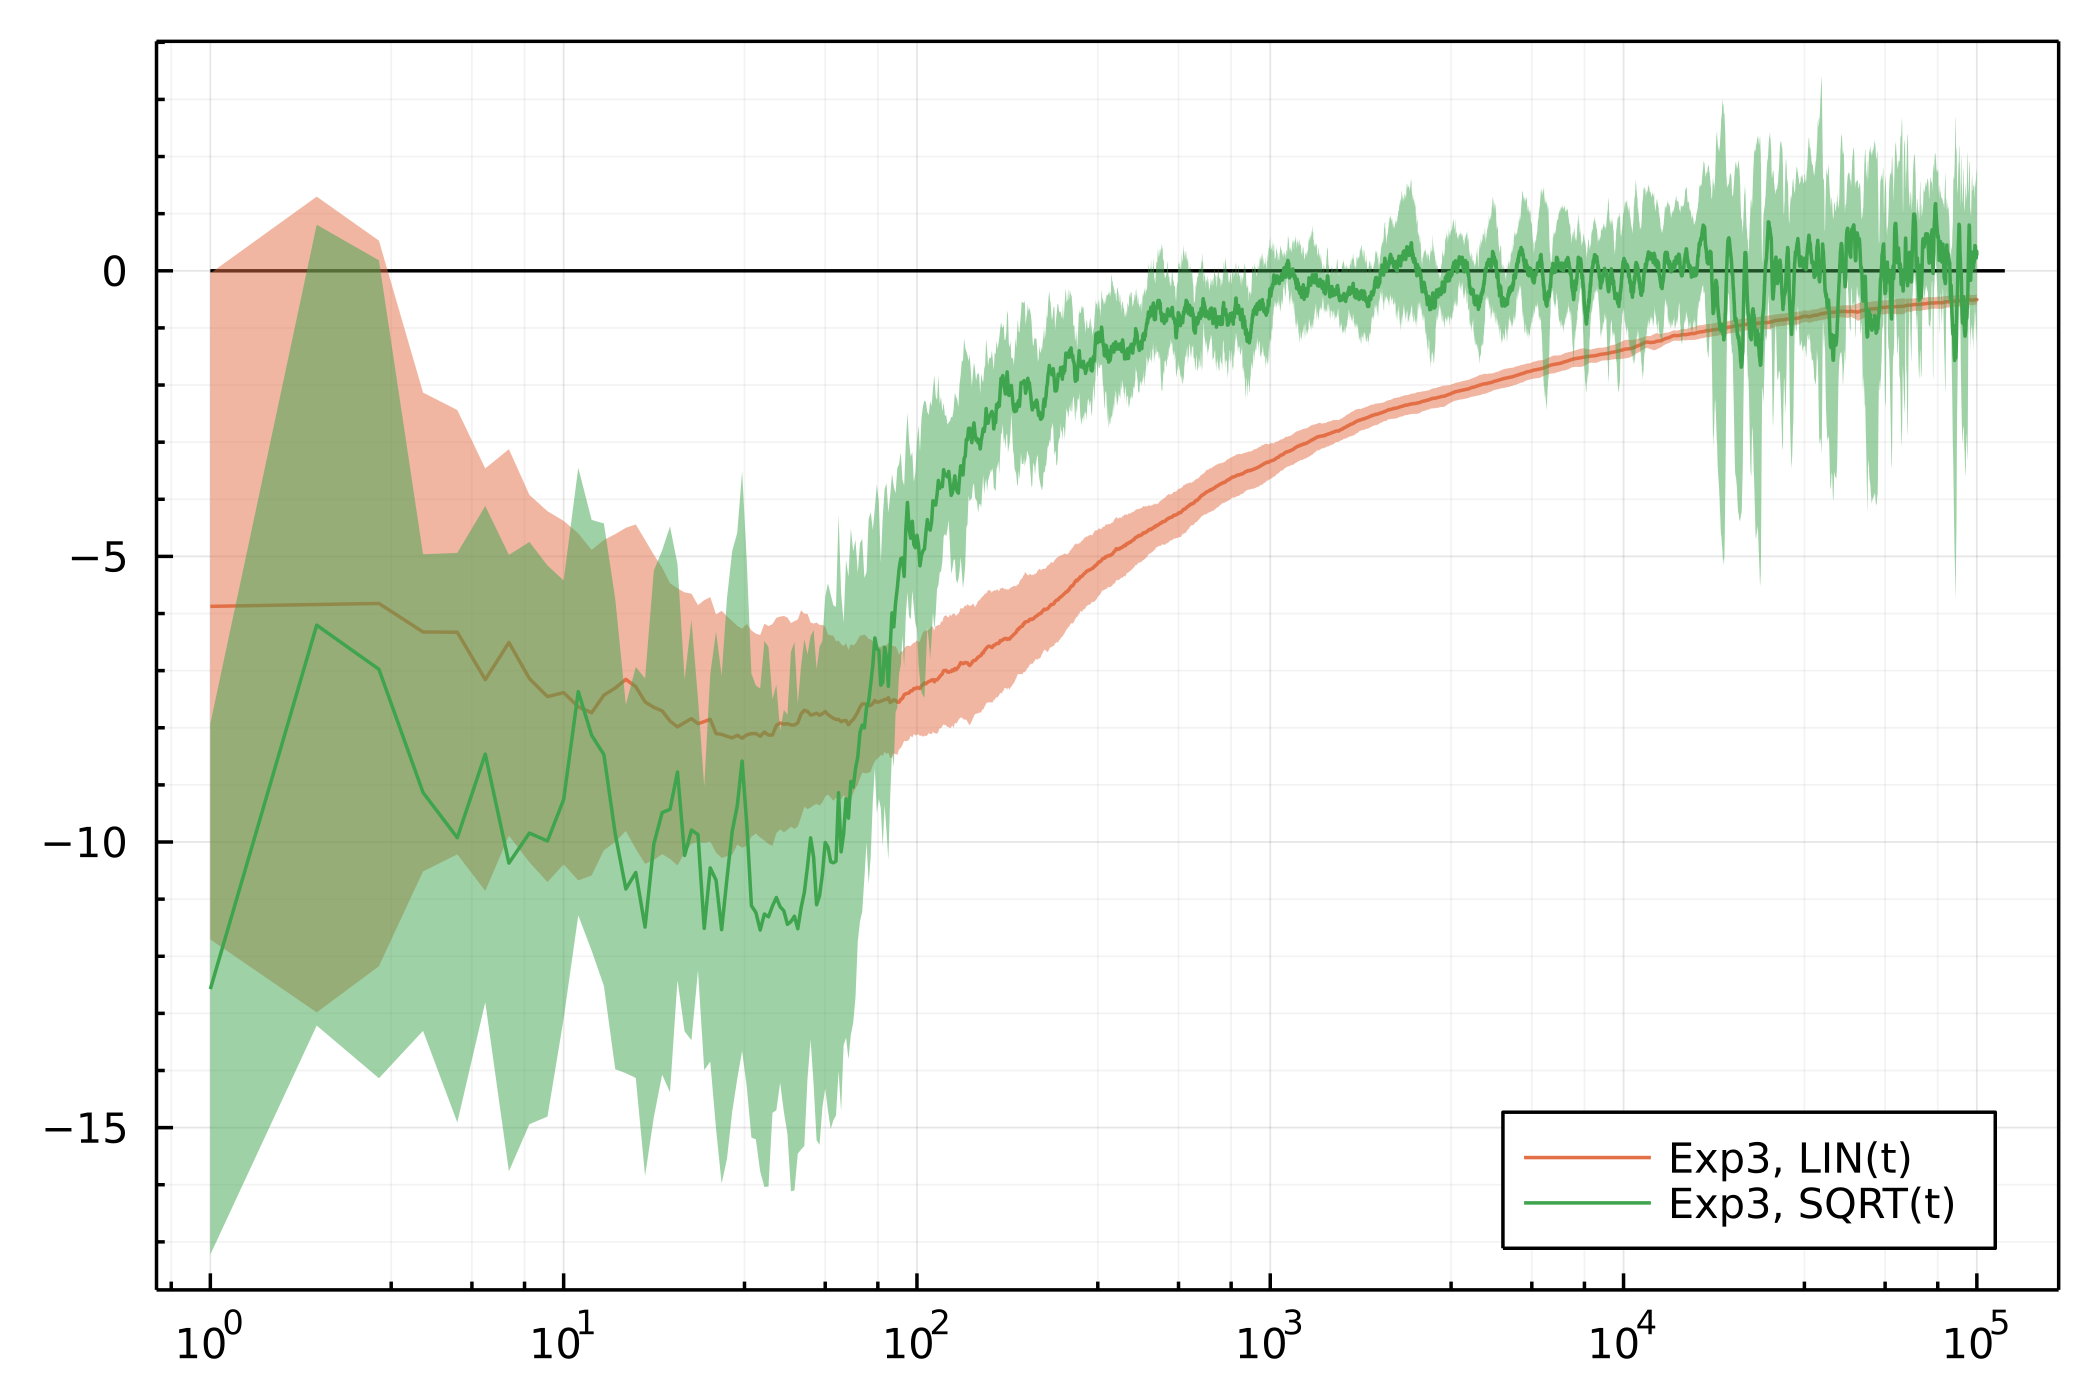
\includegraphics[width=1\textwidth]{sg/exp3/tag_3_01_Exp3_LinT_SqrtT_3_3.png}
        \caption{\tagname{3}{01} in a state $s = \left(3, 3\right)$}
        \label{apx:sgexp:exp3:fig:tag301:33}
    \end{subfigure}
    \begin{subfigure}[t]{0.45\linewidth}
        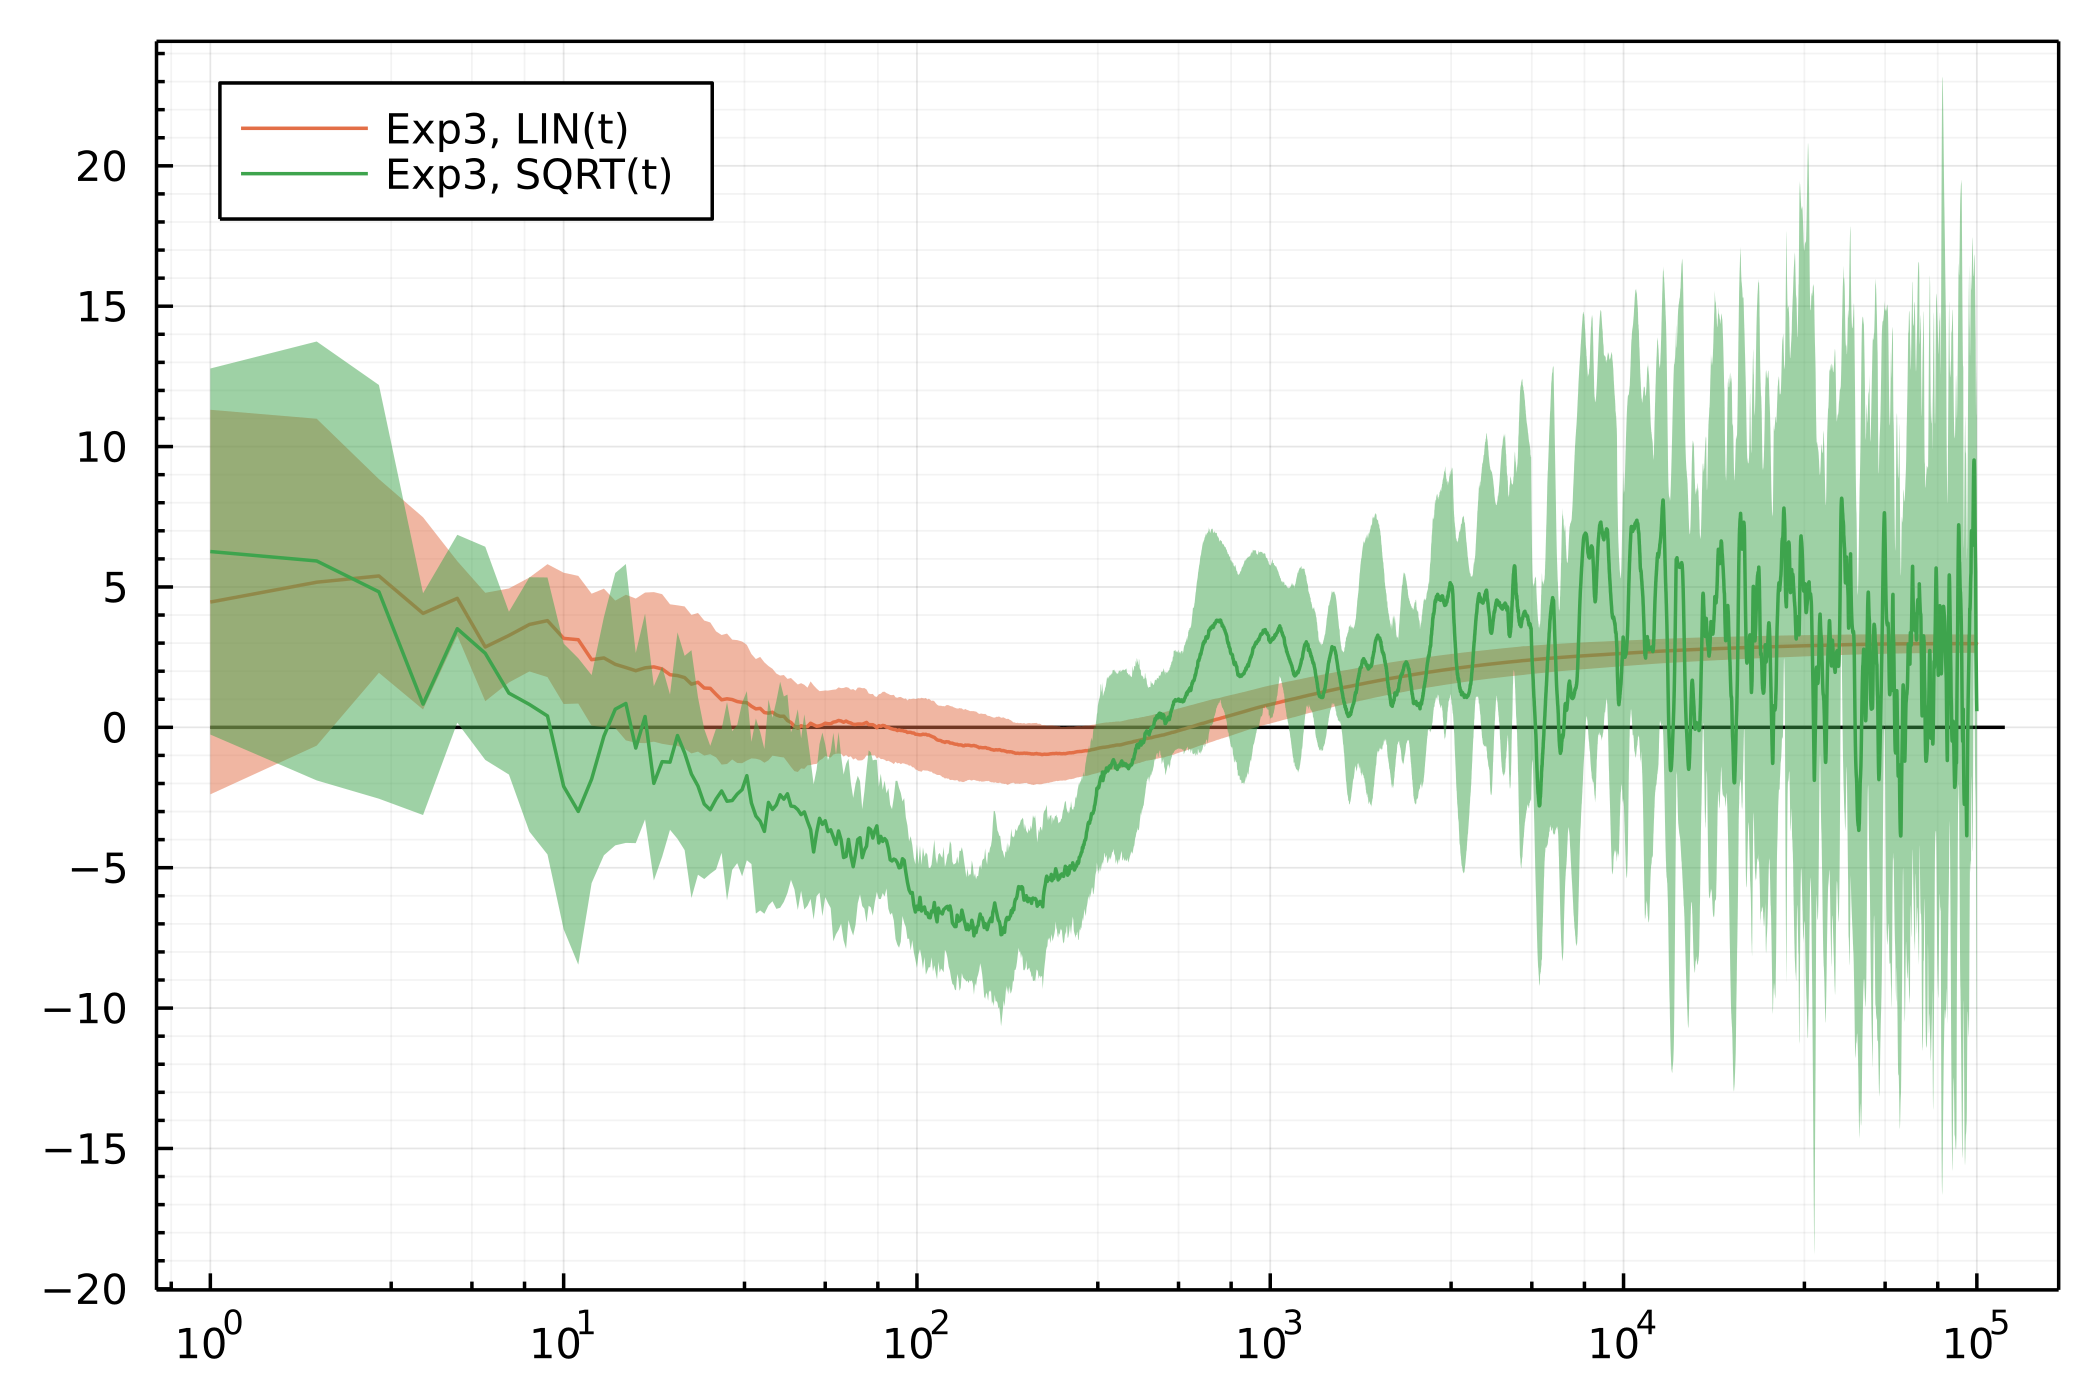
\includegraphics[width=1\textwidth]{sg/exp3/tag_3_02_Exp3_LinT_SqrtT_1_4.png}
        \caption{\tagname{3}{02} in a state $s = \left(1, 4\right)$}
        \label{apx:sgexp:exp3:fig:tag302:24}
    \end{subfigure}
    \hfill
    \begin{subfigure}[t]{0.45\linewidth}
        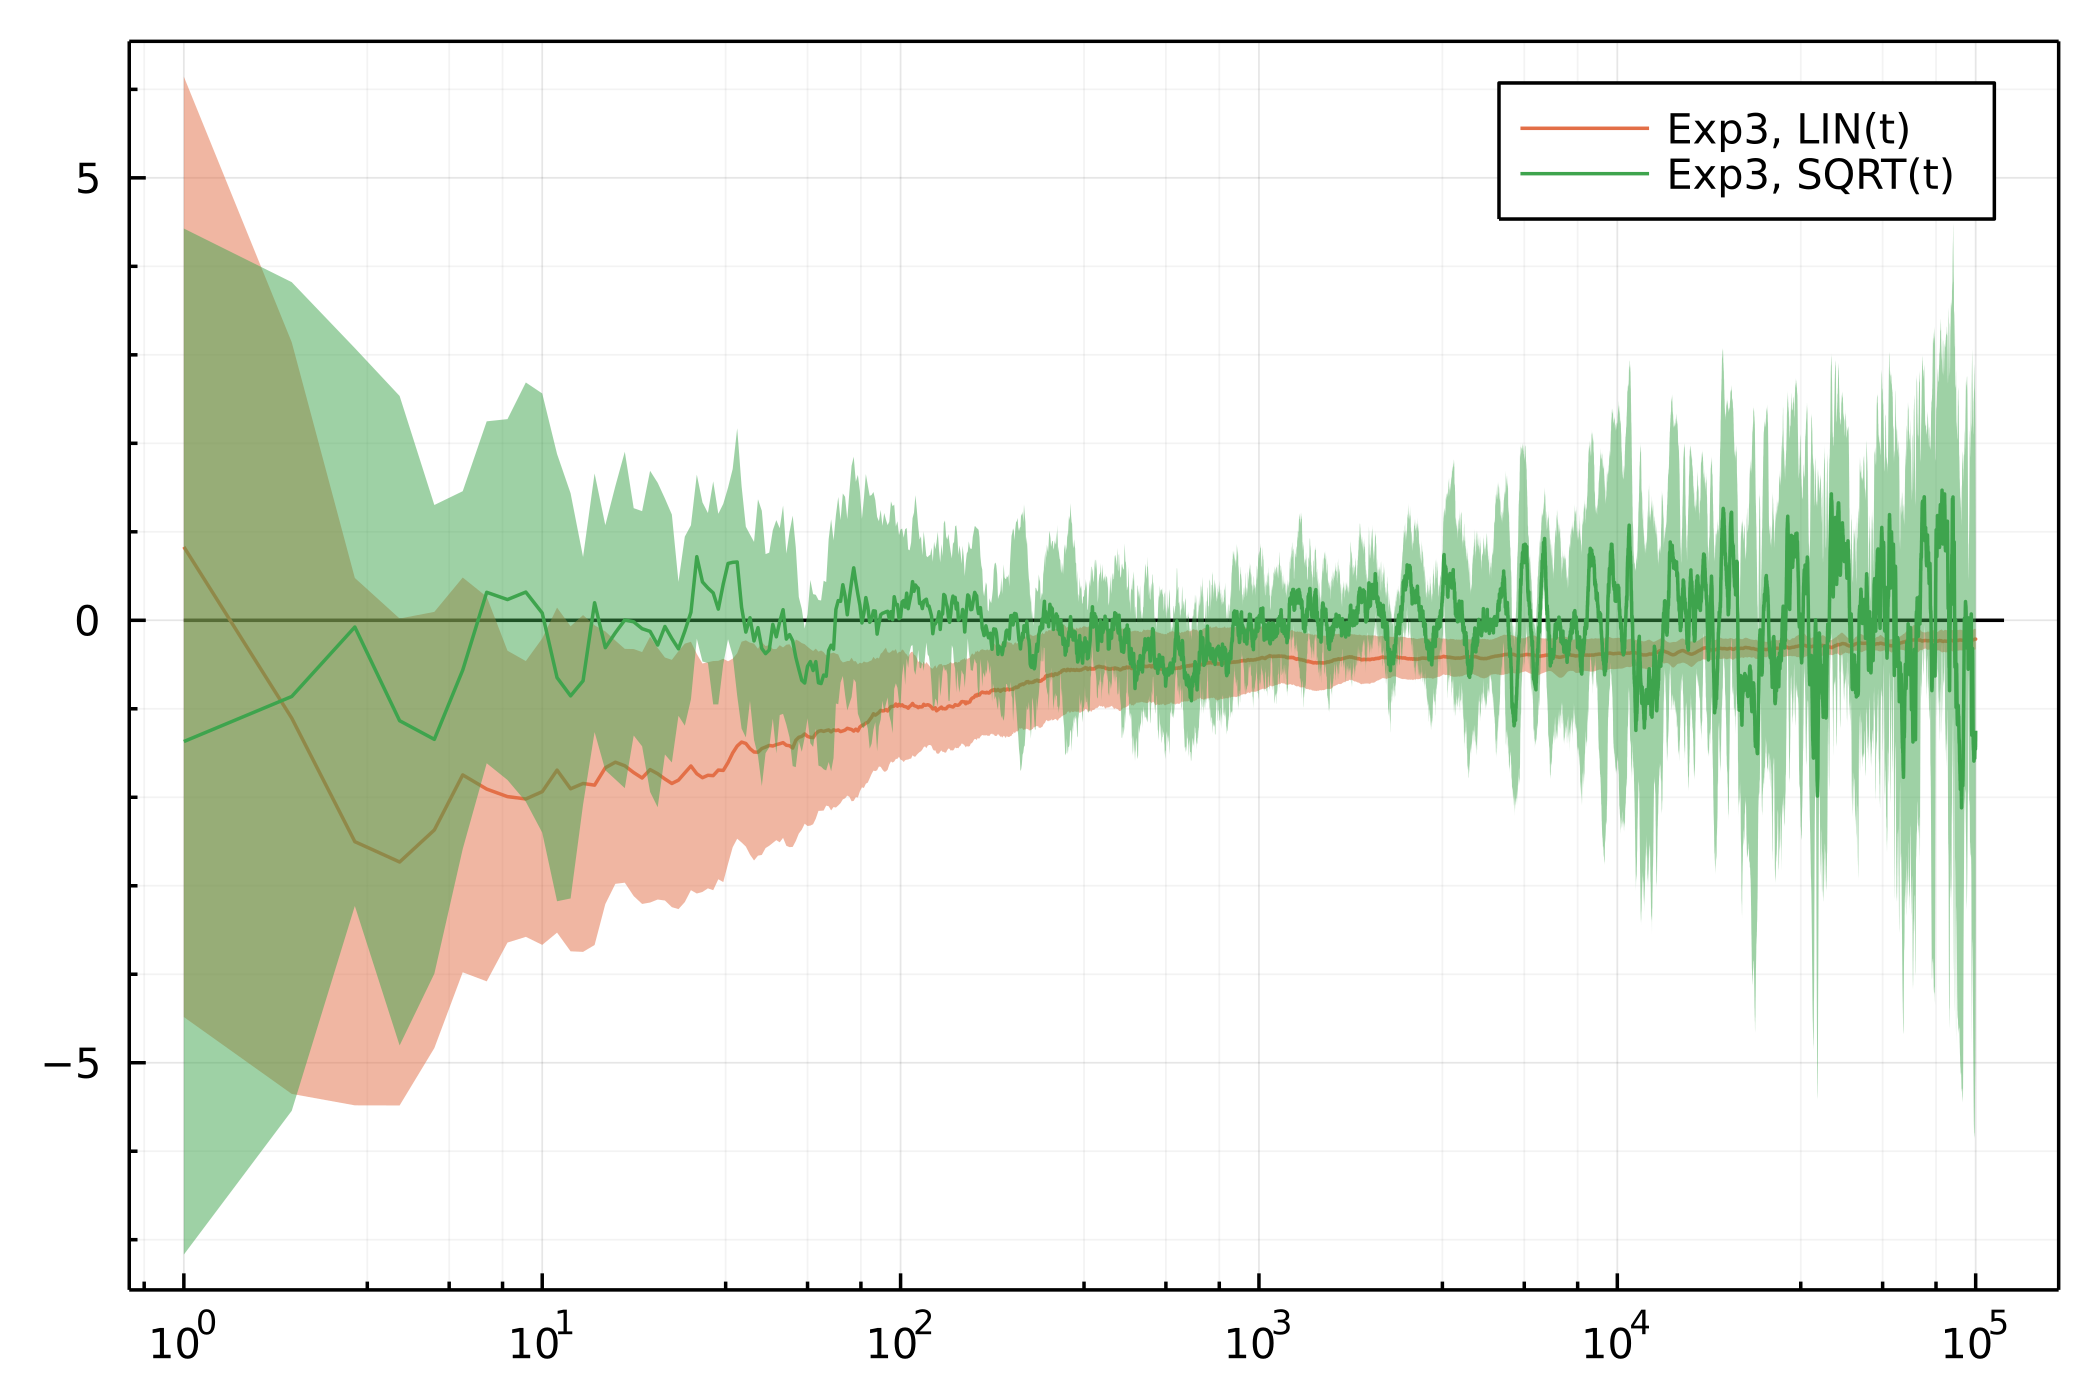
\includegraphics[width=1\textwidth]{sg/exp3/graphs_5_01_Exp3_LinT_SqrtT_3_3.png}
        \caption{\tagname{3}{02} in a state $s = \left(3, 3\right)$}
        \label{apx:sgexp:exp3:fig:chase:33}
    \end{subfigure}
    \caption[Convergence of the Exp3 algorithm depending on the step functions $\lint$ and $\sqrtt$]{
        These graphs display different convergence courses of the Exp3 algorithm in combination with either $\lint$ or $\sqrtt$ on two \textbf{Tag} instances in states where the optimal strategy is mixed.
        The graphs show dependence of deviation from the true value on the iterations $t$ of the bandit iteration algorithm.
    }
    \label{apx:sgexp:exp3:fig}
\end{figure}
The first one \reffig{apx:sgexp:exp3:fig:tag301:27}, is the easiest with a pure strategy optimum and the Exp3 algorithm converges to this value.
In this specific case, the $\sqrtt$ step again increases speed of convergence.

The rest of the examples are states, where mixed strategies has to be used to find the optima.
Clearly, the $\lint$ step can find this value, even though slowly.
The $\sqrtt$ step, on the other hand, reaches the value quicker but then oscillates around it with high amplitude.

This could be caused by computing the probability from the sums of so far received rewards in the exponential.
Moreover, the bandit samples from these computed probabilities, so the explorative power is quite strong.
Then, one such value which was then divided by the low probability of choosing the corresponding action can shift the sums in such a way that the learned probability of selection changes largely.

It can be said, that the $\sqrtt$ step function is not very appropriate for the Exp3 algorithm as the fluctuations influence the resulting values gravely.
On the other hand, these values appear centred around the 0 deviation, so their mean could be taken as the optimal value.

\end{document}
